\chapter{Método Proposto}



% -.~.-.~.-.~.-.~.-.~.-.~.-.~.-.~.-.~.-.~.-.~.-
\section{Visão geral}

O método proposto pode ser dividido em 5 etapas:
%
\begin{enumerate}
  \item Modelo dinâmico do Robô;
  \item Modelo dinâmico da Base;
  \item Modelo dinâmico acoplado da Base com Robô;
  \item Ensaio Experimental para obtenção de parâmetros modais da Base;
  \item Tratamento dos resultados e cálculo dos erros teóricos.
\end{enumerate}

Os modelos dinâmicos -- robô, base e acoplado -- são realizados com auxílio do
\textit{software} de álgebra computacional Maple, utilizando as rotinas do
Sophia. Estas ferramentas oferecem uma forma prática e sistemática de modelar um
sistema multicorpos de qualquer número de graus de liberdade e se chegar às
equações de movimento, pelo método de Kane. 

O MBS do robô é apresentado na seção~\ref{sec::modelorobo} que representa o
modelo do manipulador sobre uma base ideal, ou perfeitamente rígida, já que sua
origem não possui nenhum grau de liberdade. Nesta seção é demonstrada a
utilização do Sophia-Maple traduzindo o modelo teórico para sintaxe utilizada
pelo programa, com o objetivo também de exemplificar a modelagem sistemática de
um sistema MBS. Nas seções seguintes entretanto, não é
demonstrada a sintaxe do Sophia-Maple, no intuito de não tornar o texto
repetitivo. Os códigos completos do Sophia-Maple estão disponíveis no
Anexo\todo{Incluir ref do anexo - Sophia-Maple}.

Com o MSB do robô realiza-se, portanto, as simulações dinâmicas das trajetórias
``ideais'', ou seja, que seriam obtidas numa base perfeitamente rígida. Este
resultado permitirá a comparação das posições, velocidades e orientações ideais
com as obtidas pelo modelo acoplado.

A base é modelada na seção~\ref{sec::base}, onde é apresentado o método para
obter sua matriz de rigidez por meio de Análise por Elementos Finitos (AEF's),
utilizando o \textit{software} Autodesk Simulation.
Também é apresentado o modelo de Amortecimento de Rayleigh, também chamado de
Amortecimento Proporcional, que estima-se a matriz de amortecimento da base por
meio de apenas dois parâmetros, $\alpha$ e $\beta$, proporcionais às matrizes de
inércia e de rigidez, respectivamente.

Para calcular $\alpha$ e $\beta$ é realizado ensaio de vibrações em um modelo
físico da base. Na seção~\ref{sec::experimento} é demonstrado como obter, dos
dados experimentais, os parâmetros modais de uma estrutura, tais como
frequências naturais, modos de vibração e amortecimento. O experimento é feito
pela instrumentação da estrutura com acelerômetros e excitação com martelo
instrumentado. Os dados são tratados para obter as Funções de Resposta em
Frequência (FRF's) e então estimar seus parâmetros modais. Os valores de
$\alpha$ e $\beta$ são então calculados e utilizados no modelo da base para
fornecer a matriz de amortecimento da estrutura.

Na seção~\ref{sec::acoplado} o MBS acoplado robô e base é apresentado. Neste
caso, considera-se os 6 graus de liberdade da base (3 tranlações e 3 rotações) e
os 5 graus de liberdade associados às juntas do manipulador, formando um sistema
de 11 gdl. É simulada a mesma trajetória fornecida no modelo rígido, com o
objetivo de comparar os resultados de posição, velocidade e orientação da
ferramenta quando o robô opera sobre uma base rígida em relação a mesma operação
do robô sobre base flexível. São então verificados os efeitos da elasticidade da
base sobre os parâmetros controlados do processo sendo executado.

A Figura~\ref{fig::visgeral} ilustra uma visão geral do método proposto
facilitando a visualização das relações entre os modelos. 

\begin{figure}[h]
	\centering 
 	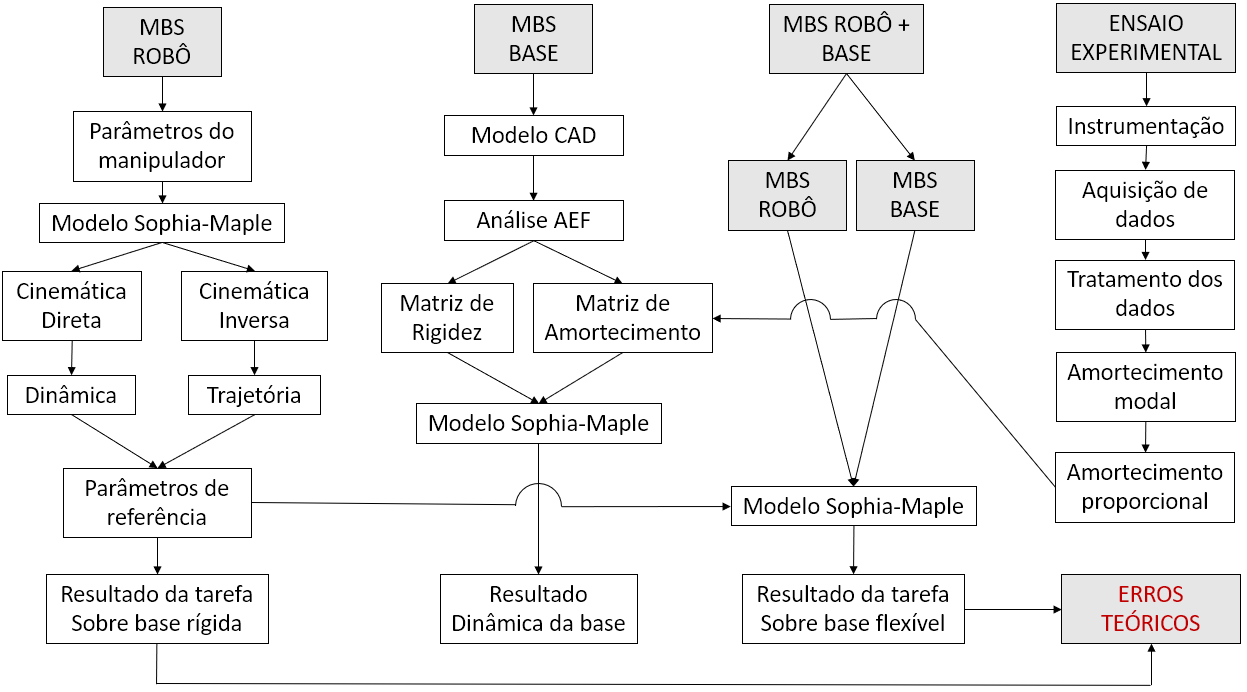
\includegraphics[width=0.95\textwidth]{figs/visgeral}
 	\caption{Diagrama da visão geral do método}
 	\label{fig::visgeral}
\end{figure}



% -.~.-.~.-.~.-.~.-.~.-.~.-.~.-.~.-.~.-.~.-.~.-
\section{Modelo do robô} \label{sec::modelorobo}

Nesta seção, são detalhados os procedimentos para representar o manipulador
robótico como um conjunto MBS e utilizá-lo para simular as trajetórias
referentes a uma determinada tarefa. O manipulador será descrito pelo conjunto
de Sistemas de Coordenadas (SC's) referente a cada uma de suas juntas, pelas
distâncias entre os SC's e posição dos centros de massa de cada elo, e pelos
parâmetros de massa e momento de inércia de cada elo. Os elos do robô e a
ferramenta acoplada no efetuador representam cada corpo do sistema MBS. A
modelagem do manipulador é simplificada utilizando as rotinas de CAS
desenvolvida especialmente para MBS, o Sophia, assim como a notação algébrica de
Lesser, apresentada na seção~\ref{sec::sophia-kane}.

\subsection{Descrição do braço robótico} \label{sec::descricao_mh12}

O manipulador escolhido para estudo é o mesmo que será utilizado no projeto EMMA
para revestimento de superfícies metálicas por HVOF. Trata-se de um robô
comercial modelo MH12, da série MOTOMAN, fabricado pela Yaskawa Motoman
(Figura~\ref{fig::mh12_foto}).

\begin{figure}[h]
    \centering
    \begin{subfigure}[b]{0.3\textwidth}
        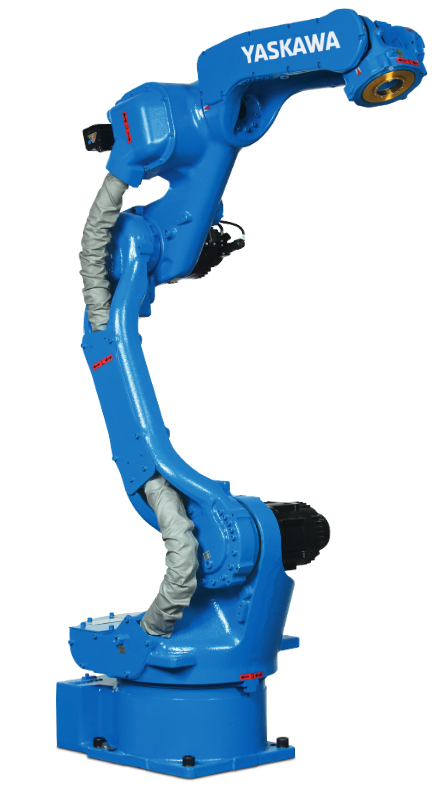
\includegraphics[width=\textwidth]{figs/mh12_foto}
        \caption{MOTOMAN MH12. \\Fonte: adaptada de}
        \label{fig::mh12_foto}
    \end{subfigure}
    \quad %add desired spacing between images, e. g. ~, \quad, \qquad, \hfill
    % etc.
      %(or a blank line to force the subfigure onto a new line)
    \begin{subfigure}[b]{0.5\textwidth}
        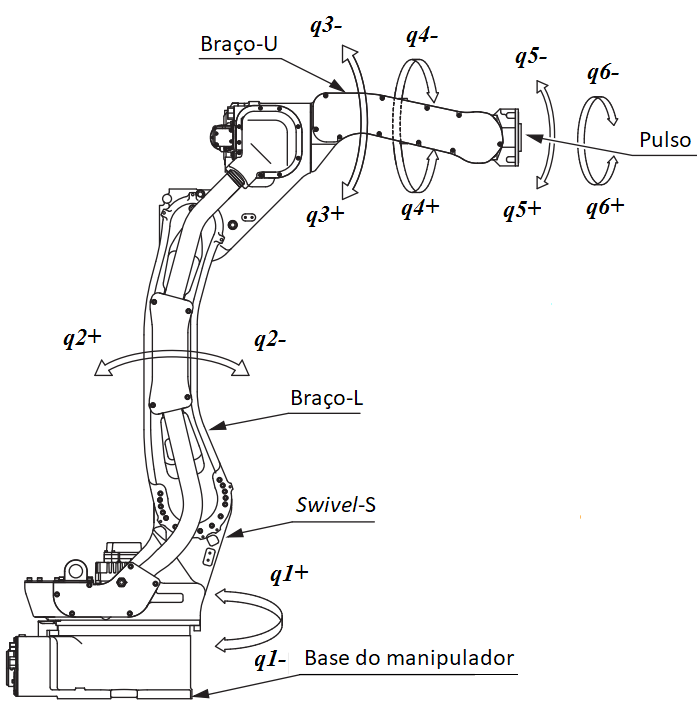
\includegraphics[width=\textwidth]{figs/mh12_diagram}
        \caption{Diagrama dos elos e juntas. \\Fonte: adaptada de}
        \label{fig::mh12_diagram}
    \end{subfigure}
    \caption{Manipulador robótico para modelo}\label{fig::resumo_mh12}
    \todo[inline]{Inncluir referências das figuras - MH12 specsheet}
\end{figure}

\begin{table}[h]
\centering
\caption{Sistemas de coordenadas, elos e coordenadas generalizadas}
\label{tab::resumo_mh12}
\begin{tabular}{@{}clc@{}}
\toprule
SC & Elo              & \multicolumn{1}{l}{Coord. gen. associada} \\ \midrule
Z  & Pedestal do robô & -                                         \\
S  & \textit{Swivel}  & q1                                        \\
L  & Braço inferior   & q2                                        \\
U  & Braço superior   & q3                                        \\
R  & Braço de rolagem & q4                                        \\
B  & Pulso            & q5                                        \\
T  & Efetuador        & q6                                        \\ \bottomrule
\end{tabular}
\end{table}

Este robô é um braço antropomórfico de 6 juntas rotacionais e portanto 6 graus
de liberdade (6 gdl), contendo o último elo um porta-ferramentas que suporta uma
carga útil de até 12 kg. A Figura~\ref{fig::mh12_diagram} apresenta os nomes dos
elos e coordenadas generalizadas associados a cada um dos sistemas de
coordenadas e são resumidos na Tabela~\ref{tab::resumo_mh12}.

O alcance horizontal deste manipulador chega a 1,440~m, e vertical a
2,511~m. Estão representados no diagrama do espaço de trabalho na
Figura~\ref{fig::workspace} em que a área sombreada é formada por todos os
pontos alcançáveis pelo manipulador, dentro dos limites de cada junta.

\begin{figure}[h]
	\centering 
 	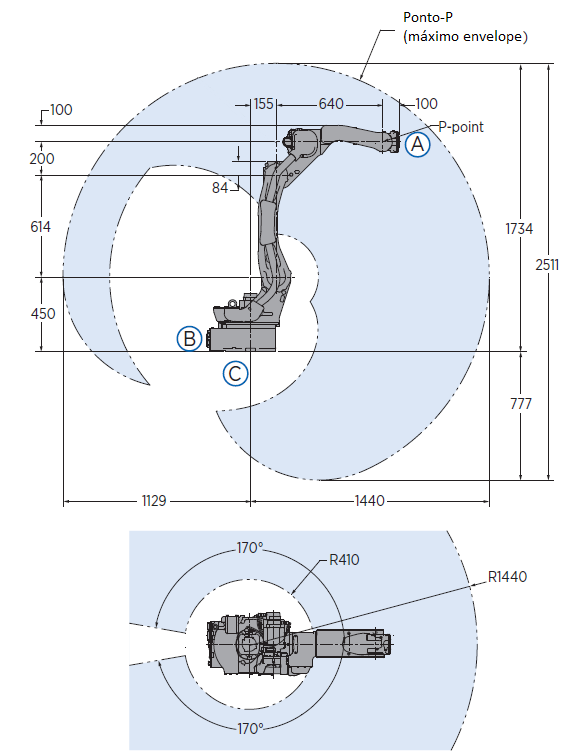
\includegraphics[width=0.7\textwidth]{figs/workspace}
 	\caption[Vistas lateral e superior do espaço de trabalho]{Vistas lateral e
 	superior do espaço de trabalho. \\Fonte: adaptada de}
 		\todo[inline]{Inncluir referência da figura - MH12 specsheet}
 	\label{fig::workspace}
\end{figure}

Conforme discutido na seção~\ref{sec::manind}, este tipo de braço robótico
permite desacoplar o sistema em 2 sub-problemas: posicionamento e orientação.
Logo, para simplificar o modelo e o cálculo da cinemática inversa, serão consideradas
as 3 primeiras juntas para posicionamento e 3 últimas (pulso esférico) para
orientação da ferramenta.

A última junta, no efetuador, tem a finalidade de orientar a ferramenta em torno
do seu eixo axial. Como o processo de revestimento por HVOF independe desta
orientação, esta junta \emph{não será incluída}, mantendo este acoplamento
rígido, o que transforma os dois últimos elos em apenas um corpo.
Como resultado, tem-se um sistema de 5 gdl.


\subsection{Cinemática Direta}\label{sec::dkin}

Como foi discutido na seção~\ref{sec::cinematica}, o procedimento mais utilizado
para a modelagem cinemática de manipuladores robóticos é o método dos parâmetros
de Denavit-Hartenberg (parâmetros D-H). Apesar de sua popularidade e vasta
utilização na modelagem cinemética de manipuladores variados, este método possui
regras que acabam restringindo uma livre escolha dos sistemas de coordenadas e
as direções dos eixos de referência. Dependendo da geometria do robô, pode ser
uma tarefa trabalhosa definir os parâmetros e referenciais mais convenientes, e
que resultem em um sistema final simplificado.

Um maior controle sobre a escolha dos referenciais e dos parâmetros da geometria
pode reduzir significativamente o custo computacional do modelo.
Neste sentido, o Sophia-Maple é uma ferramenta mais flexível, que permite, ao
usuário, total liberdade sobre a escolha dos referenciais, sem nenhum aumento de
complexidade de modelagem. Uma escolha estratégica da posição e orientação dos
sistemas de coordenadas pode resultar em equações cinemáticas e transformações de
referenciais mais simplificadas. Neste trabalho serão utilizadads as rotinas do
Sophia para modelagem da cinemática direta do manipulador robótico.

\subsubsection{Sistemas de Coordenadas e Transformações Homogêneas}

A primeira etapa para obter-se as equações cinemáticas será definir o sistema de
coordenadas fixo em cada elo do robô. A Figura~\ref{fig::scs} é um modelo CAD do
manipulador e apresenta a posição de cada SC, na sua configuração inicial.

\begin{figure}[h]
    \centering
    \begin{subfigure}[b]{0.20\textwidth}
        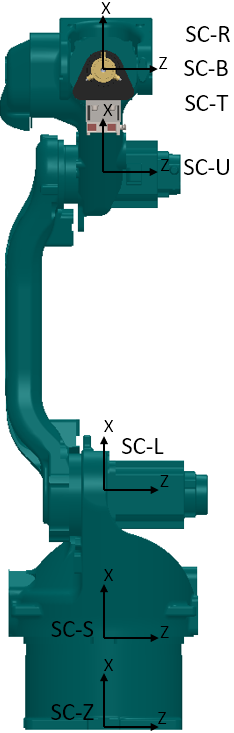
\includegraphics[width=\textwidth]{figs/sc_front}
        \caption{Vista frontal}
        \label{fig::sc_front}
    \end{subfigure}
    \quad %add desired spacing between images, e. g. ~, \quad, \qquad, \hfill
    % etc.
      %(or a blank line to force the subfigure onto a new line)
    \begin{subfigure}[b]{0.7\textwidth}
        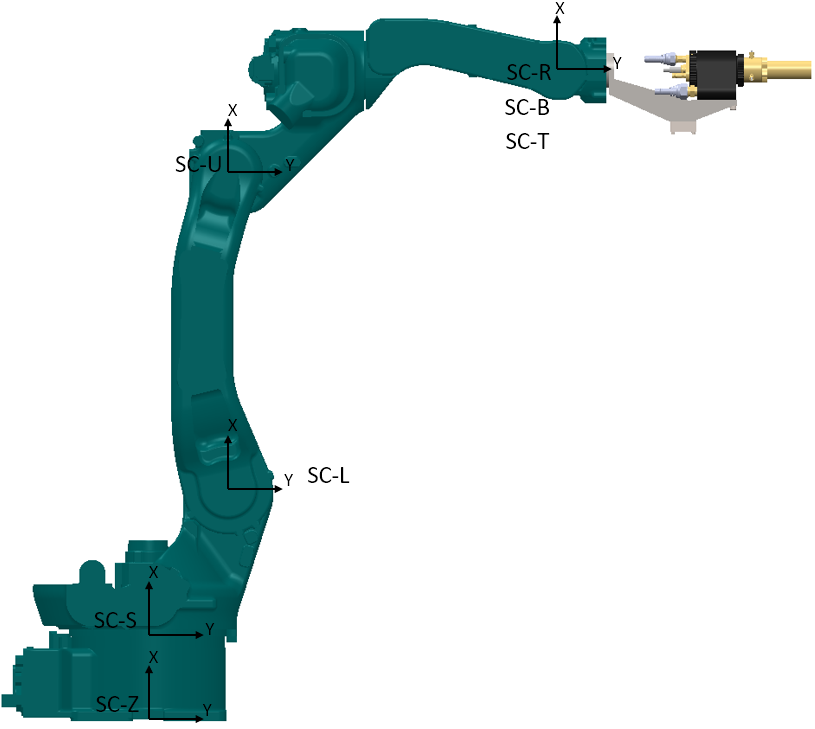
\includegraphics[width=\textwidth]{figs/sc_lat}
        \caption{Vista lateral}
        \label{fig::sc_lat}
    \end{subfigure}
    \caption{Sistemas de coordenadas do robô}\label{fig::scs}
\end{figure}

Na vista frontal (Figura~\ref{fig::sc_front}) nota-se que foi escolhida uma
configuração em que todos os SC's estivessem no mesmo plano xz. Outra observação
é que os SC's R, B e T estão fixados no mesmo ponto. que representa a origem do
``pulso'' do braço robótico. Estas considerações reduzem a quantidade de termos
das equações cinemáticas. Também terão grande impacto no cálculo da cinemática
inversa, como será visto na seção~\ref{sec::ikin_mh12}.

Logo, pode-se escrever as relações entre estes referenciais em termos das
coordenadas generalizadas do sistema, para obter as transformações entre cada
SC. No Sophia-Maple isto é feito com o uso da função \texttt{chainSimpRot}, da
seguinte forma:

\medskip \noindent {\tt > chainSimpRot( [Z,S,1,q1], [S,L,3,q2], [L,U,3,q3],
[U,R,2,q4], [R,B,3,q5], [B,T,2,q6] )} \medskip 

Esta função cria as matrizes de rotação entre os referenciais do sistema,
informando a cada transformação, o eixo de rotação
(onde 1=X, 2=Y e 3=Z) e a coordenada generalizada associada
(q1,~\ldots~,q6). Foi utilizada a forma de coordenadas relativas entre cada SC.

Como exemplo, considere o termo {\tt [L,U,3,q3]}. Representa uma rotação de um
ângulo q3, do SC-U em relação ao SC-L, em torno do eixo Z.
Logo, a matriz Transformação Homogênea entre o referencial inercial Z e o braço
superior U seria:
%
$$ R_{Z}^{U} = R_{Z}^{S} R_{S}^{L} R_{L}^{U} $$
%
A função \texttt{Rmx} do Sophia-Maple retorna a matriz de rotação entre quaisquer
sistemas de coordenadas. No Sophia-Maple, escreve-se:

\medskip \noindent {\tt > Rmx(Z,U)} \medskip 

E obtém-se o resultado:
%
$$ R_{Z}^{U} = \left( \begin {array}{ccc} {\it c2}\,{\it c3}-{\it s2}\,{\it
s3}&-{ \it c2}\,{\it s3}-{\it s2}\,{\it c3}&0\\ \noalign{\medskip}{\it c1}\,{
\it c2}\,{\it s3}+{\it c1}\,{\it s2}\,{\it c3}&{\it c1}\,{\it c2}\,{
\it c3}-{\it c1}\,{\it s2}\,{\it s3}&-{\it s1}\\ \noalign{\medskip}{
\it s1}\,{\it c2}\,{\it s3}+{\it s1}\,{\it s2}\,{\it c3}&{\it s1}\,{
\it c2}\,{\it c3}-{\it s1}\,{\it s2}\,{\it s3}&{\it c1}\end {array}
 \right) $$
 %
 A matriz acima foi escrita em notação trigonométrica simplificada, em que c1,
 s1, ,c2, s2, \ldots, e assim por diante, representam as funções senos e
 cossenos dos ângulos das coordenadas generalizadas q1, \ldots, q5. Para melhor
 visualização das matrizes e equações, esta notação será utilizada em todo o
 trabalho.
 
\subsubsection{Vetores posição e centros de massa}

A segunda etapa é definir os vetores posição dos centros de massa de cada corpo.
Para isso, define-se auxiliarmente os vetores posição entre cada sistema de
coordenada, desde o referencial inercial SC-Z até o efetuador em SC-T, de
acordo com a equação~\ref{eq::posjnutas}.

Logo, de maneira geral, pode-se escrever a posição de qualquer ponto pela
seguinte relação:
%
\begin{align}
	^{Z}\mathbf{p}^{k} &= ~^{Z}\mathbf{p}^{k-1} + ~^{k-1}\mathbf{p}^{k}
	\label{eq::posjnutas} \\
	^{Z}\mathbf{pcm}^{k} &= ~^{Z}\mathbf{pcm}^{k-1} + ~^{k}\mathbf{pcm}^k
	\label{eq::pcm}
\end{align}
%
Onde $^{Z}\mathbf{p}^{k}$ é o vetor posição do referencial $k$ em relação ao
referencial inercial $Z$ e analogamente $^{Z}\mathbf{pcm}^{k}$ é o vetor
posição do centro de massa do corpo $k$, tal que $k$ varia em \{S,L,U,B,T\},
sistemas de coordenadas do robô.
No Sophia-Maple é utilizada a notação de Lesser, por meio dos \texttt{Evectors},
para representar esses vetores, como descrito na seção~\ref{sec::sophia-kane}.

\medskip \noindent {\tt > pZ:= Evector(0,0,0,Z)} \\
\noindent {\tt > for k from corpo[1] to corpo[6] do \\
\indent p||k:= p||{k-1} \&++ Evector(p||{k-1}||{k}||x, p||{k-1}||{k}||y,
\indent p||{k-1}||{k}||z, k-1) \\
end do:} \medskip 

E para os centros de massa:

\medskip \noindent {\tt > for k from corpo[1] to corpo[6] do \\
\indent pcm||k:= p||{k} \&++ Evector(pcm||{k}||x, pcm||{k}||y, pcm||{k}||z, k)
\\ end do:} \medskip 

A Figura~\ref{fig::amb3D} apresenta o ambiente de simulação 3D, que é utilizado
para facilitar a visualização do posicionamento e movimento das juntas e elos do
robô. Defidos os pontos de origem de cada referencial, representa-se os elos do
manipulador por uma linha colorida entre os SC's. A ferramenta acoplada é
representada por uma linha que se estende desde a origem do pulso até sua
extremidade.

Neste ambiente 3D é possível fornecer qualquer configuração de juntas e
obter-se um resultado visual de posicionamento e orientação dos elos. A
Figura~\ref{fig::amb3D_posA} ilustra o resultado para a configuração inicial do
do robô, $q1 = \ldots = q6 = 0$; e a Figura~\ref{fig::amb3D_posB} para a
configuração $q1 = \ldots = q6 = {-}^{\pi}/_2$.

\begin{figure}[h]
    \centering
    \begin{subfigure}[b]{0.4\textwidth}
        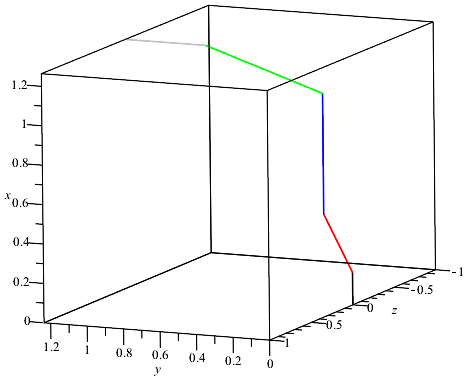
\includegraphics[width=\textwidth]{figs/amb3D_posA}
        \caption{Configuração inicial}
        \label{fig::amb3D_posA}
    \end{subfigure}
    \quad %add desired spacing between images, e. g. ~, \quad, \qquad, \hfill
    % etc.
      %(or a blank line to force the subfigure onto a new line)
    \begin{subfigure}[b]{0.45\textwidth}
        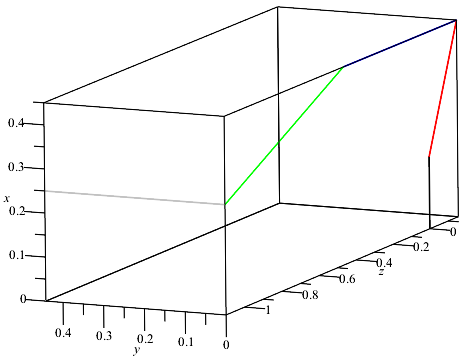
\includegraphics[width=\textwidth]{figs/amb3D_posB}
        \caption{Configuração $q1 = \ldots = q6 = {-}^{\pi}/_2$}
        \label{fig::amb3D_posB}
    \end{subfigure}
    \caption{Ambiente 3D de visualização do robô}\label{fig::amb3D}
\end{figure}

\subsubsection{Velocidades}

As velocidades dos centros de massa de cada corpo são calculadas como a derivada
do vetor posição com respeito ao referencial inercial. Logo, a derivada da
equação~\ref{eq::pcm} em Z:
%
\begin{equation} \label{eq::veloc}
	\mathbf{v}^{k} = \frac{^{Z}\mathrm{d} }{\mathrm{d} t}
	\mathbf{pcm}^{k} 
\end{equation}
%
O Sophia-Maple possui um poderoso conjunto de rotinas para diferenciação dos
\texttt{Evectors} com relação ao referencial inercial, por meio da função
\texttt{cdft}, que reconhece automaticamente o referencial em que cada vetor
está descrito e realiza o cálculo diferencial vetorial. Logo, pode-se escrever o
seguinte comando para definir as velocidades de acordo com a
equação~\ref{eq::veloc}:

\medskip \noindent {\tt > for k from corpo[1] to corpo[6] do \\
\indent v||k:= cdft(pcm||{k}, Z) \\
end do:} \medskip 

As velocidades angulares serão a taxa de variação angular das matrizes de
rotação entre os referenciais. Serão definidas as velocidades angulares de cada
corpo em relação ao referencial inercial. Conforme apresentado na
seção~\ref{sec::cinematica} pode-se escrever a velocidade angular de uma matriz
rotação $R(t)$ como:
%
\begin{equation} \label{eq::velang}
	\frac{\mathrm{d} R}{\mathrm{d} t} = S \cdot R(t)
\end{equation}
%
Onde $S$ é o tensor velocidade angular associado a $\omega$.
%
\begin{align}
% eq1
& S = \begin{pmatrix}
0				& -\omega_{z}(t)	& \omega_{y}(t) \\ 
\omega_{z}(t)	& 0					& -\omega_{x}(t) \\ 
-\omega_{y}(t)	& \omega_{x}(t)		& 0
\end{pmatrix} \\
% eq2
& \boldsymbol{\omega} = [\omega_{x}, \omega_{y}, \omega_{z}]^{T}
\end{align}
%
No Sophia-Maple o tensor $S$ pode ser calculado através da função
\&\texttt{VtoD}. Por exemplo, o tensor entre os referenciais SC-L e SC-S seria:
%
$$
S_{L}^{Z} = \left( \begin {array}{ccc} 0&-{\it q2t}&-\sin \left( {\it q2}
 \right) {\it q1t}\\ \noalign{\medskip}{\it q2t}&0&-\cos \left( {\it 
q2} \right) {\it q1t}\\ \noalign{\medskip}\sin \left( {\it q2}
 \right) {\it q1t}&\cos \left( {\it q2} \right) {\it q1t}&0
\end {array} \right)
$$
%
Porém, pode-se ainda fazer o uso da função \texttt{aV} que
calcula diretamente o vetor velocidade angular $^{A}\omega^{B}$ entre dois
referenciais. O que retornaria o seguinte vetor:
%
$$
^{Z}\boldsymbol{\omega}^{L} = [-{\it q1t},\sin \left( {\it q1} \right) {\it q2t},-\cos
\left( {\it q1} \right) {\it q2t}]
$$
%
No caso do manipulador, são calculadas as velocidades de cada corpo em relação
ao referencial Z. São definidos da seguinte forma:

\medskip \noindent {\tt > for k from corpo[1] to corpo[6] do \\
\indent w||k:= aV(Z, corpo[k]) \\
end do:} \medskip 

Podemos finalmente escrever o vetor Velocidades Generalizadas, que nada mais é
que um \texttt{Kvector} que fornece a lista de \texttt{Evectors} referente às
velocidades lineares e angulares calculadas. Logo, o vetor velocidades
generalizadas tem a seguinte forma:
%
\begin{equation}
	\mathbf{v}_{g} = [ \mathbf{v}^{S},\ldots, \mathbf{v}^{T}, \boldsymbol{\omega}^{S},\ldots,
	\boldsymbol{\omega}^{T}, 12]
\end{equation}
%
Onde cada termo do \texttt{Kvector} é um \texttt{Evector} da velocidade
generalizada.
Por fim, o último termo representa a quantidade de \texttt{Evectors} que formam o
\texttt{Kvector}.

\subsubsection{Hiperplano tangente}

Uma vez que as velocidades generalizadas foram definidas pode-se obter o
conjunto de vetores tangentes, pelo cálculo das velocidades parciais, que formam
o chamado hiperplano tangente.
Este plano é uma generalização da superfície que restringe o movimento do
sistema multicorpo e é obtido pela diferenciação das velocidades com respeito
às coordenadas generalizadas, conforme visto na seção~\ref{sec::cinematica}. As
velocidades parciais são calculadas pela expressão das velocidades
generalizadas, na equação~\ref{eq::velgen}. O termo explicitado na
equação~\ref{eq::tau} define o vetor tangente associado a i-ésima coordenada
generalizada.
%
\begin{gather}
%eq1
	^{R}\mathbf{v} = \frac{\mathrm{d} \mathbf{r}}{\mathrm{d} t} = \sum_{i}^{n}
	\dot{q_{i}} \frac{\partial r}{\partial q_{i}} + \frac{\mathrm{d}
	q_{i}}{\mathrm{d} t} \label{eq::velgen}\\
%eq2
	\dot{q_{i}} \frac{\partial r}{\partial q_{i}} = \tau_{i} \label{eq::tau}
\end{gather}
%
A função \texttt{KMtangents} do Sophia-Maple obtém os termos que formam os
vetores tangentes em \texttt{Kvectors} para cada coordenada generalizada. O
conjunto que forma o hiperplano tangente introduz uma estrutura do Sophia, dos
super \texttt{Kvectors}, ou \texttt{SKVector}. Esta estrutura facilitará a
projeção das equações dinâmicas no hiperplano tangente. Logo, para o manipulador
escreve-se:

\medskip \noindent {\tt > tau:= KMtangents(vK,u,6):} \medskip 


\subsection{Dinâmica}

Definida a cinemática direta do manipulador, deseja-se obter as forças de
inércia e externas generalizadas que fornecerão as equações de movimento do
sistema. Nesta seção primeiramente são introduzidos os parâmetros de inércia de
cada corpo do manipulador e como foram obtidos.

\subsubsection{Parâmetros de inércia do manipulador robótico}

Os parâmetros de inércia são a massa e o momento de inércia de cada corpo do
sistema. É importante notar que não é possível obter um modelo dinâmico preciso
apenas com as informações contidas nos manuais e fichas técnicas do manipulador
robótico. Infelizmente os parâmetros de inércia individuais de cada corpo não
são fornecidos pelos fabricantes e, portanto, serão estimados pelo método a
seguir.

Do manual do MOTOMAN MH12\todo{incluir ref: manual mh12}, tem-se que a massa
total do robô é de 130~kg. Também é disponibilizado, diretamente pelo
fabricante, um modelo CAD com ótimo detalhamento de cada corpo individualmente.

O programa SolidWorks foi utilizado para obter informações importantes para a
estimativa dos parâmetros de inércia. Nele é possível obter o volume de cada elo
em separado. Com isso, pode-se calcular uma massa específica média do robô, de
acordo com a equação~\ref{eq::rho}.
\begin{align}
	\rho_{m} = M_{total}\sum_{corpo[i]}^{corpo[n]} V_{i} \label{eq::rho} \qquad & ,
	i = Z,S,L,U,R,B,T
\end{align}
%
Em seguida, estima-se a massa de cada corpo, calculada pelo produto da massa
específica média $\rho_{m}$ e o volume, de acordo com a
equação~\ref{eq::massai}.
%
\begin{align}
	m_{i} = \rho_{m} \cdot V_{i} \label{eq::massai} \qquad &, i =
	Z,S,L,U,R,B,T
\end{align}
%
A massa da ferramenta acoplada ao efetuador foi obtida de forma precisa,
pelo projeto CAD do suporte, e informação do fabricante do dispositivo
HVOF.
A Tabela~\ref{tab::massa_mh12} apresenta os resultados da massa estimada em cada
corpo:
%
\begin{table}[h]
\centering
\caption{Resultado do cálculo da massa de cada corpo}
\label{tab::massa_mh12}
\begin{tabular}{@{}clc@{}}
\toprule
\textbf{Corpo}                      & \textbf{Volume} [$m^3$] & \multicolumn{1}{l}{\textbf{Massa} [kg]} \\ \midrule 
Z 									& 0,01595         & 40,5							   \\
S                                   & 0,01443         & 36,7                               \\
L                                   & 0,00579         & 14,7                               \\
U                                   & 0,00997         & 25,3                               \\
R                                   & 0,00399         & 10,1                               \\
B                                   & 0,00100         & 2,5                                \\
T                                   & 0,00005         & 0,13                               \\
Ferramenta                          & -		          & 5,97							   \\ \midrule
\textbf{Volume total}~$=$           & 0,05119        & \multicolumn{1}{c}{$m^3$}	       \\
\multicolumn{1}{r}{\textbf{$\rho_m =$}} & 2540          &
\multicolumn{1}{c}{$kg/{m^3}$}     \\ \bottomrule
\end{tabular}
\end{table}
%

Para este modelo dinâmico, não será utilizada a última junta do robô, como foi
explicado na seção~\ref{sec::descricao_mh12}, de forma que pode-se considerar os
corpos ``B, T e Ferramenta'' como um único corpo. Assim, as propriedades de
massa e momento de inércia podem ser somadas e condensadas em uma única
descrição. 

A partir daqui, estes 3 últimos corpos serão tratadaos como um único corpo e
será utilizada a denominação do corpo B para representar esse conjunto.

Do CAD do MH12 também é possível extrair as as posições do centro de massa e
momentos de inércia de cada elo.
Como se considerou que a massa de cada elo é distribuida homogeneamente no seu
volume, isto resulta numa posição estimada do centro de massa. A
Tabela~\ref{tab::resumo_cm} resume os valores encontrados para a posição do
centro de massa com respeito ao referencial de cada elo e a
Figura~\ref{fig::pcm_mh12} ilustra no modelo CAD a posição aproximada.

\begin{figure}[h]
	\centering 
 	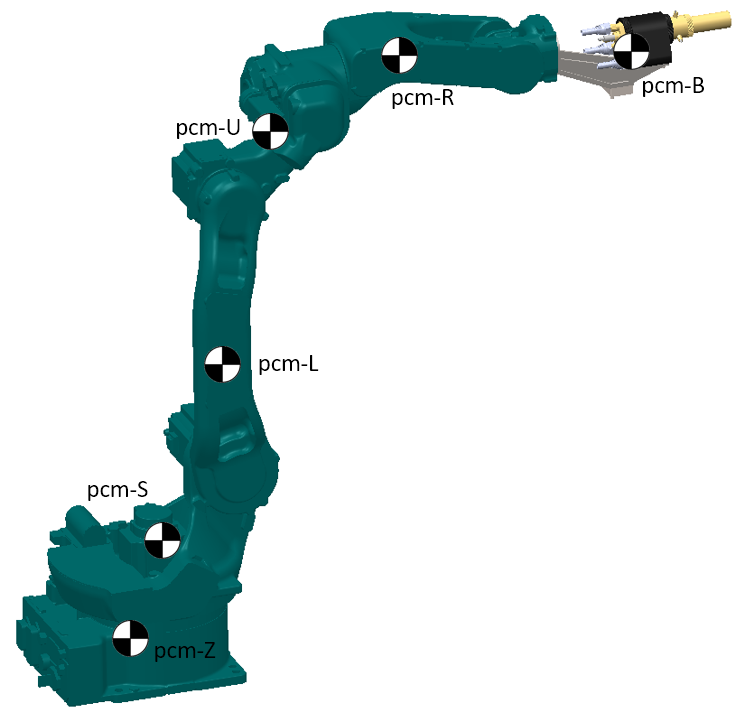
\includegraphics[width=0.7\textwidth]{figs/pcm_mh12}
 	\caption{Posição aproximada dos centros de massa}
 	\label{fig::pcm_mh12}
\end{figure}

%
\begin{table}[h] \centering
\caption{Posição do centro de massa}
\label{tab::resumo_cm}
\begin{tabular}{@{}cccc@{}}
\toprule
\textbf{Corpo} & \textbf{x [m]} & \textbf{y [m]} & \textbf{z [m]} \\ \midrule
Z              & 0,079      & -0,050     & 0,000      \\
S              & 0,124      & 0,027      & 0,008      \\
L              & 0,281      & -0,025     & -0,115     \\
U              & 0,123      & 0,115      & -0,025     \\
R              & 0,039      & -0,224     & 0,004      \\
B              & -0,011     & 0,146      & 0,000      \\ \bottomrule
\end{tabular}
\end{table}
%

O modelo CAD também calcula os momentos de inércia de cada elo obtidos no
centro de massa e alinhados ao sistema de coordenadas de referência daquele elo.
O resultado do cálculo dos momentos de inércia de cada elo são apresentados a
seguir.
%
\begin{align*}
InZ &=& \left( \begin {array}{ccc}  0,811& 0,293& 0,091\\ \noalign{\medskip}
 0,293& 0,695& 0,064\\ \noalign{\medskip} 0,091& 0,064& 0,923
\end {array} \right) & \quad InS &=& \left( \begin {array}{ccc}  0,811& 0,293& 0,091\\ \noalign{\medskip}
 0,293& 0,695& 0,064\\ \noalign{\medskip} 0,091& 0,064& 0,923
\end {array} \right) \\
InL &=&  \left( \begin {array}{ccc}  0,051&-
0,008&- 0,032 \\ \noalign{\medskip}- 0,008& 0,791& 0,011\\ \noalign{\medskip}- 0,032
& 0,011& 0,798\end {array} \right) & \quad InU &=& \left( \begin {array}{ccc} 
0,314& 0,149&- 0,077\\ \noalign{\medskip} 0,149& 0,367&- 0,057\\ \noalign{\medskip}- 0,077&- 0,057& 0,418
\end {array} \right) \\
InR &=&  \left( \begin {array}{ccc}  0,173&-
0,014& 0,001\\ \noalign{\medskip} - 0,014& 0,052& 0,004\\ \noalign{\medskip} 0,001& 0,004& 0,148
\end {array} \right) & \quad InB &=&  \left( \begin {array}{ccc}  0,235&- 0,018& 0,0\\ \noalign{\medskip}-
 0,018& 0,039& 0,0\\ \noalign{\medskip} 0,0& 0,0& 0,243\end {array}
 \right)
\end{align*}
%
No Sophia-Maple estes tensores são construidos com a função
\texttt{EinertiaDyad}, que aproveita o fato dos tensores de inércia serem
simétricos e recebe 6 argumentos para os termos da matriz e um para especificar
o sistema de coordenadas de referência em que foi obtido o tensor. Define-se
portanto cada tensor da seguinte forma:

\medskip \noindent {\tt > for i from corpo[1] to corpo[6] do \\
\indent In||(corpo[i]):= EinertiaDyad( \\
\indent In||(corpo[i])||11, In||(corpo[i])||22, \\
\indent In||(corpo[i])||33, In||(corpo[i])||12, \\
\indent In||(corpo[i])||13, In||(corpo[i])||23, sc[i]) \\
end do:}

\subsubsection{Quantidade de Movimento e Quantidade de Movimento Angular}

Para o cálculo das forças de inércia, calcula-se a Quantidade de Movimento $G$ e
a Quantidade de Movimento Angular $H$, para cada corpo, de acordo com as
equações~\ref{eq::qntmov} e \ref{eq::qntmovang}.
%
\begin{align}
%eq1
	\mathbf{G}_{k} &= m_{k} \cdot \mathbf{v}_{k} \label{eq::qntmov} \\
%eq2	
	\mathbf{H}_{k} &= In_{k} \cdot \boldsymbol\omega^{k} \label{eq::qntmovang}
\end{align}
%

\subsubsection{Forças de Inércia}

As forças de inércia são a derivada temporal das quantidades de movimento, com
respeito ao referencial inercial Z, conforme descrito pelas
equações~\ref{eq::finG} e \ref{eq::finH}.
%
\begin{align}
%eq1
	\dot{\mathbf{G}}_{k} &= \frac{^{Z}\mathrm{d}}{\mathrm{d} t} (m_{k} \cdot
	\mathbf{v}_{k}) \label{eq::finG} \\
%eq2	
	\dot{\mathbf{H}}_{k} &= \frac{^{Z}\mathrm{d}}{\mathrm{d} t} (In_{k} \cdot
	\mathbf{\boldsymbol\omega^{k}}_{k}) \label{eq::finH}	
\end{align}
%
No Sophia-Maple, obtém-se primeiro os vetores quantidade de movimento e, em
seguida, constrói-se o \texttt{Kvector} das quantidades de movimento com a
função \texttt{KM} armazendado na variável \texttt{KMG}. Um função especial para
diferenciação de \texttt{Kvectors}, \texttt{Kfdt} é aplicada em \texttt{KMG} para
calcular os vetores das forças de inércia.

Vale notar que o Sophia-Maple adiciona um sufixo t aos termos que foram
derivados com respeito ao tempo.
Logo, as coordenadas generalizadas, q1,\ldots,qn, quando derivadas no tempo
resultam em q1t,\ldots,qnt. Este formato auxilirá a substituição destes termos
para solução das \textit{kinematic differential equations} (kde), conforme visto
na seção~\ref{sec::sophia-kane}.

O algoritmo para definir as Forças de Inércia do sistema no Sophia-Maple é o
seguinte:

\medskip \noindent {\tt > for i from 1 to 6 do \\
\indent G||corpo[i]:= m||corpo[i] \&** v||corpo[i] \\
end do: \# Define as Quantidades de Movimento}

\medskip \noindent {\tt > for i from 1 to 6 do \\
\indent H||corpo[i]:= In||corpo[i] \&** w||corpo[i] \\
end do: \# Define as Quantidades de Movimento Angular}

\medskip \noindent {\tt > KMG:= subs(kde, KM[G||corpo, H||corpo]): \\
\# Define o Kvector das Quantidades de Movimento generalizadas}

\medskip \noindent {\tt > FIN:= subs(kde, Z Kfdt KMG): \\
\# Define o Kvector das Forças de Inércia}


\subsubsection{Forças Externas}

Uma das vantagens do método de Kane é não ser necessário avaliar as forças
internas, ou de restrição entre os corpos dos sistema. O motivo é que, ao se
projetarem as equações de equilíbrio dinâmico no hiperplano tangente, essas
forças desaparecem.

Logo, apenas as forças externas precisam ser modeladas para obter as equações de
movimento. No modelo do braço robótico, estas forças são o peso, os torques das
juntas e os torques de controle PID, em cada elo.

A força peso atua aplicada ao centro de massa de cada corpo \textit{k} e é calculada
pela equação~\ref{eq::peso}:
%
\begin{equation}
	\mathbf{Peso}_{k} = m_{k} \cdot \mathbf{g} \label{eq::peso}
\end{equation}
%
Onde $\mathbf{g}$ refere-se ao vetor da aceleração da gravidade, que atua sempre
no sentido de $-X$ no referencial inercial Z. É definido como:
%
\begin{equation}
	\mathbf{g} = [-9,81,~0,~0]^{Z}
\end{equation}
%
Os momentos externos são formados pelos torques dos atuadores em cada junta e
também os torques de controle PID. Neste momento é válido acrescentar uma
explicação rápida sobre a modelagem do controlador PID.

\subsubsection{Parâmetros de controle PID}

Para que o robô realize uma tarefa, é necessário seguir uma trajetória
previamente planejada. Uma trajetória pode ser simplesmente um conjunto de
posições de referência de cada junta, que varia no tempo, como foi abordado na
seção~\ref{sec::ikin_traj}. A variação das posição se dá pelo acionamento dos
torques em cada junta, que deve ser controlado para seguir a trajetória
planejada. 

Os fabricantes de robôs comerciais infelizmente não fornecem detalhes sobre o
método nem os parâmetros de controle utilizados.
Com o propósito de simular o controle do manipulador decidiu-se pela
simplicidade do método de controle PID.

Os parâmetros de controle PID são formados pelas variáveis proporcional,
integral e derivativa, ou $Kp$, $Td$ e $Ti$ respectivamente. Esses parâmetros
foram sintonizados para cada junta individualmente, fazendo-se simulações de
resposta para uma função degrau de referência. Os resultados mostraram que este
método é suficiente para seguir a trajetória e manter os erros dentro de uma
margem de tolerância aceitável. Alguns dos resultados são demonstrados no
Apêndice X\todo{Incluir apêndice para resultados PID}.

Como resultado da análise, encontrou-se os melhores resultados
para o conjunto de parâmetros apresentados na\todo{atualizar parâmetros PID}
Tabela~\ref{tab::pid}:
%
\begin{table}[h]
\centering
\caption{Parâmetros de controle PID em cada junta}
\label{tab::pid}
\begin{tabular}{@{}clll@{}}
\toprule
\textbf{Junta} & \textbf{Kp [Nm]} & \textbf{Ti [Nm]} & \textbf{Td [Nm]} \\ \midrule 
S              & 400         & 80000       & 3000        \\
L              & 2000        & 500000      & 15000       \\
U              & 1200        & 400000      & 12000       \\
R              & 100         & 100000      & 1000        \\
B              & 250         & 100000      & 1000        \\ \bottomrule
\end{tabular}
\end{table}
%

Logo, define-se as equações dos torques de controle para cada junta, em função
da diferença entre os parâmetros instantâneos e os de referência em cada junta.
O subíndice $k$ representa a lista de juntas, localizada na origem de cada
sistema de coordenadas de mesmo nome, variando em \{S,L,U,R,B\} e o
subíndice $i$ o número da coordenada generalizada associada.
%
\begin{equation}
	PID_{k} = Kp(q_i-q_i{ref}) + Ti\int_{t1}^{t2} (q_i-q_i{ref})dt +
	Td(u_i-u_i{ref}) \label{eq::pid}
\end{equation}
%
No Sophia-Maple declara-se os torques de controle representados na
equação~\ref{eq::pid} da seguinte forma:

\medskip \noindent {\tt > for k from 1 to 5 do \\
		 \indent PID\_||{corpo[k]}:= Kp*(q||k - q||k||ref) + Ti*int(q||k - q||k||ref,
		 t) + Td*(u||k - u||k||ref) \\
		 end do:}

\subsubsection{Momentos Externos}

Para obter os momentos externos que atuam em cada corpo, o primeiro passo é
definir os torques que atuam em cada junta. Para eliminar os momentos causados
pelas forças \texttt{Peso}, avaliou-se os torques das juntas com respeito ao
centro de massa de cada corpo. As equações~\ref{eq::tjuntasi} a
\ref{eq::tjuntasf} descrevem os torques externos e de controle que atuam em cada
junta.
\begin{align}
	\mathbf{TjZS} &= (TZS - PID_{S})\cdot[1,~0,~0]^Z \label{eq::tjuntasi} \\
	\mathbf{TjSL} &= (TSL - PID_{L})\cdot[0,~0,~1]^S \\
	\mathbf{TjLU} &= (TLU - PID_{U})\cdot[0,~0,~1]^L \\
	\mathbf{TjUR} &= (TUR - PID_{R})\cdot[0,~1,~0]^L \\
	\mathbf{TjRB} &= (TRB - PID_{B})\cdot[0,~0,~1]^B \label{eq::tjuntasf}
\end{align}
%
As equações~\ref{eq::mexi} a \ref{eq::mexf} calculam o somatório dos momentos
externos em cada corpo. Nota-se que o torque aplicado em qualquer junta causa
um par de torques de ação e reação nos elos adjacentes. As variáveis $Mex_k$ são
grandezas vetoriais que representam o momentos externos resultante em cada
corpo.
%
\begin{align}
	\mathbf{Mex_{Z}} &= - \mathbf{TjZS } \label{eq::mexi}\\
	\mathbf{Mex_{S}} &= \mathbf{TjZS} - \mathbf{TjSL }\\
	\mathbf{Mex_{L}} &= \mathbf{TjLU }- \mathbf{TjSL }\\
	\mathbf{Mex_{U}} &= \mathbf{TjUR }- \mathbf{TjLU }\\
	\mathbf{Mex_{R}} &= \mathbf{TjRB }- \mathbf{TjUR }\\
	\mathbf{Mex_{B}} &= - \mathbf{TjRB} \label{eq::mexf}
	\end{align}
%
A Figura~\ref{fig::sisfex} ilustra, em vista explodida, o equilíbrio das forças e
momentos externos em cada elo do manipulador.
%
\begin{figure}[h]
    \centering
    \begin{subfigure}[b]{0.6\textwidth}
        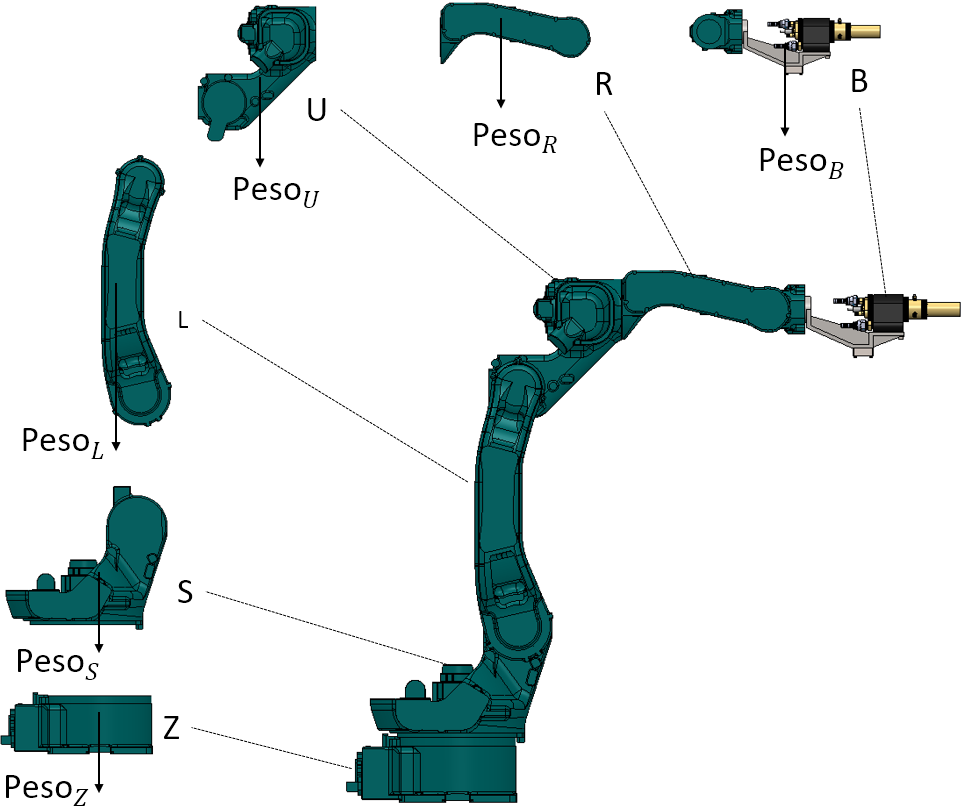
\includegraphics[width=\textwidth]{figs/forcas_ext}
        \caption{Forças externas em cada elo}
        \label{fig::fex}
    \end{subfigure}
    \quad %add desired spacing between images, e. g. ~, \quad, \qquad, \hfill
    % etc.
      %(or a blank line to force the subfigure onto a new line)
    \begin{subfigure}[b]{0.6\textwidth}
        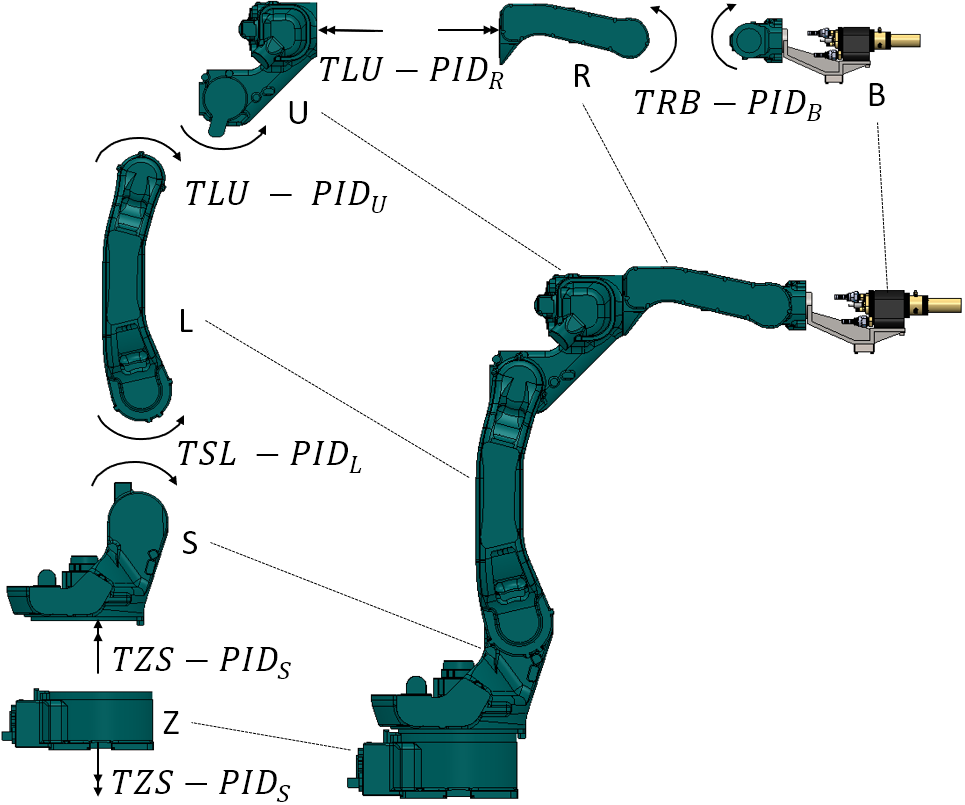
\includegraphics[width=\textwidth]{figs/mom_ext}
        \caption{Momentos externos em cada elo}
        \label{fig::mex}
    \end{subfigure}
    \caption{Sistema de forças externas}\label{fig::sisfex}
\end{figure}
%

Nota-se novamente que, pelo método de Kane, não é preciso introduzir as forças
internas, de restrição ou de contato entre os corpos, porque estas não
contribuem para as equações de movimento e desaparecem quando o sistema de
equações de equilíbrio dinâmico são projetads no hiperplano tangente, $\tau$.

No Sophia-Maple os vetores dos momentos externos resultantes são armazenadas em
\texttt{Evectors}. A sequência de equações~\ref{eq::tjuntasi} a \ref{eq::mexf}
torna-se:

\medskip \noindent {\tt > \# Torques nas juntas} \\
		 \noindent {\tt > TjZS:= Evector(TZS - PID\_S,~0,~0,~S) } \\
		 \noindent {\tt > TjSL:= Evector(0,~0,~TSL - PID\_L,~L) } \\
		 \noindent {\tt > TjLU:= Evector(0,~0,~TLU - PID\_U,~U) } \\
		 \noindent {\tt > TjUR:= Evector(0,~TUR - PID\_R,~0,~R) } \\
		 \noindent {\tt > TjRB:= Evector(0,~0,~TUR - PID\_B,~B) }

\medskip \noindent {\tt > \# Momentos externos em cada elo} \\
		 \noindent {\tt > for k from 1 to 5 do \\
		 \indent Mex||k:= Tj||{k-1}||{k}  - Tj||{k}||{k+1} \\
		 end do:} \\
		 \noindent {\tt > MexB:= - TjRB:} \medskip

		 
As forças e momentos externos podem ser agrupadas em um único vetor para
auxiliar a projeção destas em $\tau$. Novamente, faz-se uso da função
\texttt{KM}, o que retorna um \texttt{Kvector} contendo todas as forças e
momentos, descritos em cada sistema de referência.

\medskip \noindent {\tt > FEX:= KM[Fex||corpo,~Mex||corpo]:}

		 
\subsubsection{Forças de Inércia e  Forças Externas Generalizadas}

Estas são as forças externas e de inércia FEX e FIN, quando projetadas no
hiperplano tangente, $\tau$. Para a projeção, faz-se uso da função
\texttt{\&kane}, do Sophia-Maple, o que retorna as equações implícitas
generalizadas de cada corpo:

\medskip \noindent {\tt > FEXg:= tau \&kane FEX:} \\
		 \noindent {\tt > FINg:= tau \&kane FIN:}
		 
\subsubsection{Equações de Movimento}

Finalmente, as equações de movimento são formadas pelo equilíbrio dinâmico entre
as forças externas e externas generalizadas obtidas da projeção em $\tau$, de
acordo com a equação~\ref{eq::eqdin}:
%
\begin{equation}
	(FINg - FEXg)_{k} = 0 \label{eq::eqdin}
\end{equation}
%
O subíndice \textit{k} representa a lista de corpos \{Z,S,L,U,R,B\}. Como o
corpo Z está fixo no referencial inercial SC-Z, sua equação de movimento
torna-se a solução trivial $0=0$ e portanto, não fará parte do sistema. Obtém-se
então um conjunto de 5 equações de movimento, associadas aos 5 gdl do robô.

No Sophia-Maple atribui-se o conjunto de equações~\ref{eq::eqdin} à
variável \texttt{kane}, formando uma lista das equações de movimento. Portanto:

\medskip \noindent {\tt > kane:= FINg - FEXg = 0} \medskip

As equações denominadas \textit{kinematic differential equations}, ou
\texttt{kde}, completam o sistema de equações diferenciais que descrevem o
movimento do robô.
Para os 5 graus de liberdade do manipulador, tem-se 5 kde. As
equações~\ref{eq::kde5i} a \ref{eq::kde5f} descrevem o kde:
%
\begin{align}
	u_{1}(t) &= \frac{\mathrm{d} }{\mathrm{d} t}q_{1}(t) \label{eq::kde5i} \\
	u_{2}(t) &= \frac{\mathrm{d} }{\mathrm{d} t}q_{2}(t) \\
	u_{3}(t) &= \frac{\mathrm{d} }{\mathrm{d} t}q_{3}(t) \\
	u_{4}(t) &= \frac{\mathrm{d} }{\mathrm{d} t}q_{4}(t) \\
	u_{5}(t) &= \frac{\mathrm{d} }{\mathrm{d} t}q_{5}(t) \label{eq::kde5f}	
\end{align}
%
Somando-se esse sistema às equações de movimento e atribuindo à variável
\texttt{eq\_mov}, no Sophia-Maple:

\medskip \noindent {\tt > eq\_mov:= kane union kde:} \medskip

Logo, tem-se um sistema de 10 equações diferenciais ordinárias, não-lineares
(equações~\ref{eq::eqdin} a \ref{eq::kde5f}), cujas incógnitas são as
coordenadas generalizadas $q_{1}(t),\ldots, q_{5}(t)$ e as velocidades angulares
$u_{1}(t),\ldots, u_{5}(t)$.

Vale ressaltar que, para o sistema de apenas 5 equações de movimento simbólicas
associadas aos 5 graus de liberdade, as expressões são extensas demais para
serem representadas neste texto, o que ocuparia diversas páginas e obviamente
não traria nenhum valor à discussão deste tópico. Por isso, limita-se a
representação do sistema à equação~\ref{eq::eqdin}.

A função \texttt{cost} do Maple retorna o número de operações algébricas e de
funções de uma determinada equação ou sistema de equações fornecendo um
parâmetro para o usuário avaliar o tamanho das expressões e o custo
computacional do modelo.
Para se ter uma ideia, o custo do sistema de equações de movimento, representado
na forma puramente simbólica em \ref{eq::eqdin}, tem  a seguinte estrutura:
\begin{equation*}
	18171\,{\it additions}+59804\,{\it multiplications}+39998\,{\it 
functions}
\end{equation*}
%
Porém, até então não foram substituidos os parâmetros numéricos do robô, nas
variáveis simbólicas . Este procedimento simplifica o sistema, porque muitos
termos são zerados. Além disso, é possível fazer uso da função \texttt{simplify}
do Maple, que é um poderoso conjunto de rotinas para simplificação algébrica de
expressões. Fazendo uso desta função e da substituição dos parâmetros numéricos
nas equações de movimento, obtemos o novo custo algébrico das equações:
%
\begin{equation*}
	5676\,{\it additions}+6992\,{\it multiplications}+1835\,{\it functions}
\end{equation*}
%
Nota-se a grande vantagem de realizar este procedimento, porque ao reduzir-se
drasticamente o número de termos e funções, reduz-se também o custo
computacional e por consequência o tempo para o cálculo da solução.

\subsubsection{Problema de Valor Inicial -- PVI}

Para resolver o sistema diferencial é necessário fornecer as condições de
contorno do problema. Como as equações estão no domínio do tempo, são fornecidas
as condições iniciais das variáveis de estado $q_{1}(0),\ldots, q_{5}(0)$ e
$u_{1}(t),\ldots, u_{5}(0)$.

Será adotado neste modelo que qualquer trajetória será iniciada a partir da
configuração incial do robô, ou seja:
%
\begin{equation}
	q_{1}(0) = \ldots = q_{5}(0) = u_{1}(0) = \ldots = u_{5}(0) = 0
	\label{eq::condini}
\end{equation}
%
O sistema completo será portanto formado pelas 10 equações de movimento
diferenciais e não lineares (\ref{eq::eqdin} a \ref{eq::kde5f}), com as 10
equações de valor incial definidas em~\ref{eq::condini}.

Para definir esse sistema no Sophia-Maple, primeiro cria-se a lista com as
equações de valor inicial e então adiciona-as ao sistema, utilizando a função
\texttt{union}:

\medskip \noindent {\tt > cond\_ini:= \{seq(q||i(0) = 0, i=1..5), seq(u||i(0) =
0, i=1..5)\}} \\ 
		 \noindent {\tt > sistema:= eq\_mov union condini:} \medskip

A solução deste sistema depende ainda da definição dos seguintes parâmetros:
%
\begin{itemize}
  \item{Torques nas juntas: TZS, TSL, TLU, TUR, TRB}
  \item{Coordenadas de referência dos ângulos de juntas: 
  		\\ $q_{1}ref, q_{2}ref, q_{3}ref, q_{4}ref, q_{5}ref$}
  \item{Velocidades angulares de referências das juntas: 
  		\\ $u_{1}ref, u_{2}ref, u_{3}ref, u_{4}ref, u_{5}ref$}
\end{itemize}
%
A trajetória efetuada pelo manipulador é então consequência da solução do
sistema, para um conjunto de parâmetros fornecidos. Para realizar uma trajetória
desejada, deve-se fornecer os parâmetros de referência e torques das juntas ao
longo do tempo que resultam naquela trajetória.

Se tal trajetória é descrita pela posição e orientação da ferramenta acoplada ao
último elo do manipulador, os parâmetros das juntas, tais que a ferramenta
segue aquela trajetória, devem ser determinados pelo cálculo da Cinemática
Inversa.


\subsection{Cinemática Inversa}\label{sec::ikin_mh12}

Como o manipulador MOTOMAN MH12 é do tipo antropomórfico 6R com pulso esférico,
a modelagem da cinemática inversa se resume em encontrar os parâmetros das
juntas que satisfazem ao problema desacoplado, detalhado na
seção~\ref{sec::ikin_traj}, ou seja, as funções $q_{1}, q_{2}, q_{3}$ que
satisfazem a posição e $q_{4}, q_{5}, q_{6}$ que satisfazem a orientação da
ferramenta.

A posição final da ferramenta pode ser portanto expressa como função da posição
de sua extremidade e orientação em termos das coordenadas generalizadas, de
acordo com a equação~\ref{eq::posf}.
%
\begin{equation}
	\mathbf{x}_{f} = \begin{bmatrix}
		\mathbf{p}_{f} \\ \boldsymbol{\Phi}_{f}
	\end{bmatrix}
	\label{eq::posf}	
\end{equation}
%
\noindent onde: 
%
\begin{align}
\mathbf{p}_{f}^Z &= [x_f,y_f,z_f]^Z \\
\boldsymbol{\Phi}_{f}^Z &= [\phi,\theta,\psi]^Z
\end{align}
%

\todo[inline]{Incluir figura representando a posição e orientação final da
ferramenta}

\subsubsection{Cálculo da posição do pulso}

A primeira tarefa será calcular a posição da ferramenta em termos das
coordenadas generalizadas.
Como visto na seção~\ref{sec::ikin_traj}, pode-se expressá-la convenientemente
pela posição da origem do pulso, porque esta só depende das coordenadas $q_1, q_2$ e $q_3$.

A posição da ponta da ferramenta, $p_{f}$, é então a posição da origem do pulso,
$p_{w}$ em SC-R, somada ao vetor das dimensões da ferramenta, no referencial
SC-B:
\begin{equation}
	\mathbf{p}_{f}^Z = \mathbf{p}_{w} + [d_{x}, d_{y}, d_{z}]^B \label{eq::posf}
\end{equation}
%
Pelo desenvolvimento da cinemática direta, na seção~\ref{sec::dkin}, pode-se
expressar a posição de qualquer ponto da cadeia cinemática em um dado
referencial. Como o pulso tem origem no sistema de coordenadas SC-R, então:
%
\begin{equation} \label{eq::pwpr}
	\mathbf{p}_{w} =~^Z{\mathbf{p}}^R 
\end{equation}
%
Recorrendo às equações~\ref{eq::ikinq1} a \ref{eq::ikinq6}, desenvolvidas na
seção~\ref{sec::ikin_traj}, pelo método geométrico para a solução da cinemática
inversa deste tipo de manipulador, tem-se:
%
\begin{align*}
	q1 &= \atantwo (z_w,y_w) - \atantwo (d, \pm \sqrt{y_w^2 + z_w^2 - d^2}) \\
	q2 &= \atantwo (r,s) - \atantwo (\pm  \sqrt{1-E^2}, E) \\
	q3 &= \atantwo (\pm \sqrt{1-D^2}, D) - \frac{\pi}{2} + \atantwo (h, a3)
\end{align*}
%
Onde:
%
\begin{align*}
	D &= \frac{r^2 + s^2 -a2^2 - a3^2}{2 \cdot a2 \cdot a3} \\
	E &= - \frac{a3^2 - a2^2 - r^2 - s^2}{2 \cdot a2 \cdot \sqrt{r^2 + s^2}}
\end{align*}
%
Uma análise das expressões acima permite relacionar os termos geométricos
do robô genérico com os parâmetros fornecidos do MOTOMAN MH12. Substiui-se
portanto estes termos de acordo com as relações:
%
\begin{align}
	r &= \sqrt{x_w^2 + y_w^2 - d^2} - pSLy \\
	s &= x_w - (pZSx + pSLx) \\
	d &= 0 \\
	h &= pURx \\
	a2 &= pLUx \\
	a3n &= pURy \\
	a3 &= \sqrt{h^2 + a3n^2}
\end{align}
%
E obtém-se:
%
\begin{align}
	q1 &= \atantwo (z_w,y_w) \label{eq::q1ik} \\
	q2 &= \atantwo ( \sqrt {y_w^2 + z_w^2}- pSLy, x_w - pZSx - pSLx ) \nonumber \\
	   &- \atantwo ( \pm \sqrt {-E^2+1}, E ) \\
	q3 &= \atantwo ( \pm \sqrt {-{{\it D}}^{2}+1},{\it D} ) -\pi /2 +
\atantwo ( {\it pURx},{\it pURy} ) \label{eq::q3ik}
\end{align}
%
Onde:
%
\begin{align}
	D &= \textstyle \frac{1}{2}\,{\frac {-{{\it pLUx}}^{2}-{{\it pURx}}^{2}-{{\it
	pURy}}^{2}+ \left( \sqrt {{{\it y_w}}^{2}+{{\it z_w}}^{2}}-{\it pSLy} \right) ^{2
		}+ \left( {\it x_w}-{\it pZSx}-{\it pSLx} \right) ^{2}}{{\it pLUx}\,
		\sqrt {{{\it pURx}}^{2}+{{\it pURy}}^{2}}}} \\
	E &= \textstyle {-\frac{1}{2}\,{\frac {-{{\it pLUx}}^{2}+{{\it pURx}}^{2}+{{\it
		pURy}}^{2}- \left( \sqrt {{{\it y_w}}^{2}+{{\it z_w}}^{2}}-{\it pSLy} \right)
		^{2 }- \left( {\it x_w}-{\it pZSx}-{\it pSLx} \right) ^{2}}{{\it pLUx}\,
		\left[ \left( \sqrt {{{\it y_w}}^{2}+{{\it z_w}}^{2}}-{\it pSLy}
 		\right) ^{2}+ \left( {\it x_w}-{\it pZSx}-{\it pSLx} \right) ^{2}
 		\right]^{1/2}}}}
\end{align}
%
Determina-se portanto, pelo método geométrico, as coordenadas $q_1, q_2$ e
$q_3$ em função da posição do pulso e dos parâmetros geométricos do robô. Note que $x_w,
y_w, z_w$ são as coordenadas da posição do pulso, no referencial inercial e que
para calcular a posição da ferramenta, pela equação~\ref{eq::pwpr} precisa-se
ainda definir sua orientação.

Note-se também que existem 4 soluções para cada posição do pulso. Se
considerar-se os limites dos ângulos das juntas do robô, pode-se limitar o
número de soluções. Para exemplificar, a Figura~\ref{fig::elbowupdown} demonstra
duas soluções para a posição $\mathbf{p}_{w} = [0,7,~ 0,8,~ 0]^Z$: cotovelo para
cima em linha cheia e cotovelo para baixo em linha pontilhada.

\begin{figure}[h]
	\centering 
 	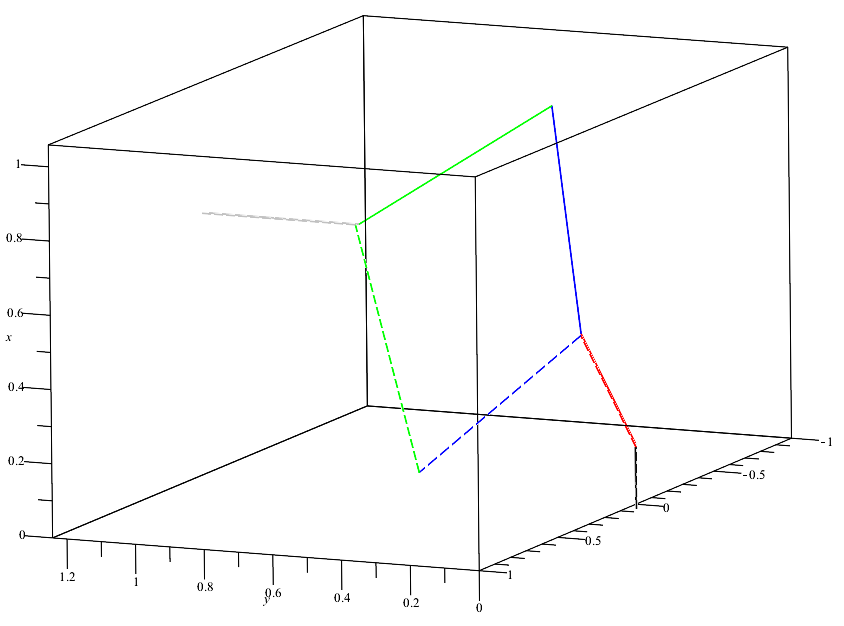
\includegraphics[width=0.75\textwidth]{figs/elbowupdown}
 	\caption{Exemplo de duas soluções possíveis para o mesmo ponto}
 	\label{fig::elbowupdown}
\end{figure}


\subsubsection{Cálculo da orientação da ferramenta}

Nesta etapa, deseja-se calcular a orientação da ferramenta, em relação ao
referencial inercial. Para isso são utilizados os ângulos $\phi,\theta,\psi$
para reresentar os ângulos de Euler das 3 rotações que orientam o referencial do
pulso na direção desejada.

Recorrendo novamente ao desenvolvimento da cinemática inversa geral para este
tipo de manipulador, da seção~\ref{sec::ikin_traj}, obteve-se da
equação~\ref{eq::rut} a relação:
%
\begin{equation*}
	R_{U}^{T} = (R_{Z}^{U})^T R_{yzy}
\end{equation*}
%
Onde $R_{zyz}$ representa a matriz rotação pelos ângulos de Euler
$\phi,\theta,\psi$, em torno dos eixos $Y,Z,Y$ respectivamente.

As matrizes de rotação $(R_{Z}^{U})^T$ e $R_{U}^{T}$ são calculadas para os
valores de $q_1, q_2$ e $q_3$ das equações~\ref{eq::q1ik} a \ref{eq::q3ik}.
Assim, a equação~\ref{eq::rutik} fornece um sistema de 9 equações e 6
incógnitas, se consideradas as funções senos e cossenos de $q_4, q_5$ e $q_6$ a serem
determinadas.
%
\begin{multline} \label{eq::rut}
%eq1
	 \left[ \begin {array}{ccc} {\it c4}\,{\it c5}\,{\it c6}-{\it s4}\,{
\it s6}&-{\it c4}\,{\it s5}&{\it c4}\,{\it c5}\,{\it s6}+{\it c6}\,{
\it s4}\\ \noalign{\medskip}{\it s5}\,{\it c6}&{\it c5}&{\it s5}\,{
\it s6}\\ \noalign{\medskip}-{\it c5}\,{\it c6}\,{\it s4}-{\it c4}\,{
\it s6}&{\it s4}\,{\it s5}&-{\it c5}\,{\it s4}\,{\it s6}+{\it c4}\,{
\it c6}\end {array} \right] = \\
%eq2
	 \left[ \begin {array}{ccc} {\it c2}\,{\it c3}-{\it s2}\,{\it s3}&-{
\it c2}\,{\it s3}-{\it s2}\,{\it c3}&0\\ \noalign{\medskip}{\it c1}\,{
\it c2}\,{\it s3}+{\it c1}\,{\it s2}\,{\it c3}&{\it c1}\,{\it c2}\,{
\it c3}-{\it c1}\,{\it s2}\,{\it s3}&-{\it s1}\\ \noalign{\medskip}{
\it s1}\,{\it c2}\,{\it s3}+{\it s1}\,{\it s2}\,{\it c3}&{\it s1}\,{
\it c2}\,{\it c3}-{\it s1}\,{\it s2}\,{\it s3}&{\it c1}\end {array}
 \right]^T \cdot \\
%eq3
	\cdot \left[ \begin {array}{ccc} c\phi \,c\theta \,c\psi -s\phi \,s\psi &-c
\phi \,s\theta &c\phi \,c\theta \,s\psi +s\phi \,c\psi 
\\ \noalign{\medskip}s\theta \,c\psi &c\theta &s\theta \,s\psi 
\\ \noalign{\medskip}-s\phi \,c\theta \,c\psi -c\phi \,s\psi &s\phi \,
s\theta &-s\phi \,c\theta \,s\psi +c\phi \,c\psi \end {array} \right] 
\end{multline}
%

Analisando o lado esquerdo da equação~\ref{eq::rut} pode-se determinar
facilmente a solução para $\cos(q5)$, porque este será diretamente o resultado
alocado no termo $[2,2]$ da matriz 3x3 resultante do lado direito da equação, ou
seja:
%
\begin{multline}
\cos(q5) = {\it c2}\,{\it c3}\,s\phi \,{\it s1}\,s\theta -s\phi \,{\it s1}\,{\it 
		s2}\,{\it s3}\,s\theta +c\phi \,{\it c2}\,{\it s3}\,s\theta +
		\\ +c\phi \,{\it c3}\,{\it s2}\,s\theta +{\it c1}\,{\it c2}\,{\it c3}\,c\theta -{
		\it c1}\,{\it s2}\,{\it s3}\,c\theta 
\end{multline}
%
E seu seno é calculado por:
%
\begin{equation}
	\sin(q5) = \sqrt{1-\cos(q5)^2}
\end{equation}
%
Logo, utilizando a relação trigonométrica, $\sin(q5)/\cos(q5) = \tan(q5)$,
e invertendo a função tangente, determina-se:
%
\begin{equation}
	q5 = \atantwo(\sqrt{1-\cos(q5)^2}, \cos(q5))
\end{equation}
%

Para determinar $q4$ analisa-se novamente a matriz $R_{U}^{T}$. Se dividir o
termo $[3,2]$,  multiplicado por $(-1)$, pelo termo $[1,2]$, dos lados esquerdo
e direito da equação~\ref{eq::rut}, obtém-se uma expressão para $\tan(q4)$.
Invertendo a função tangente para obter $q4$:
\begin{multline} 
q4 = \atantwo( {{\it c1}\,s\phi \,s\theta -{\it s1}\,c\theta} , ~
 \left[  \left( s\phi \,{\it s1}\,{\it s3}-c\phi \,{\it c3} \right) {
\it c2}+{\it s2}\, \left( {\it c3}\,s\phi \,{\it s1}+c\phi \,{\it s3}
 \right)  \right] s\theta +
 \\ +{\it c1}\,c\theta \, \left( {\it c2}\,{\it 
s3}+{\it s2}\,{\it c3} \right) 
 )
\end{multline}
%
Similarmente à solução de $q4$, mas desta vez fazendo a divisão dos termos
$[2,3]$ por $[2,1]$, dos lados esquerdo e direito da equação~\ref{eq::rut},
encontra-se $q6$:
%
\begin{equation} \label{eq::q6ik}
	q6 = \atantwo ( {s6} , {c6} )
\end{equation}
%
Onde:
%
\begin{multline*}
	s6 = -{\it c2}\,{\it c3}\,s\phi \,s\psi \,{\it s1}\,c\theta +s\phi \,s\psi 
		\,{\it s1}\,{\it s2}\,{\it s3}\,c\theta +c\phi \,c\psi \,{\it c2}\,{
		\it c3}\,{\it s1}-c\phi \,c\psi \,{\it s1}\,{\it s2}\,{\it s3} +
		\\ -c\phi \,{\it c2}\,s\psi \,{\it s3}\,c\theta -c\phi \,{\it c3}\,s\psi \,{\it 
		s2}\,c\theta +{\it c1}\,{\it c2}\,{\it c3}\,s\psi \,s\theta -{\it c1}
		\,s\psi \,{\it s2}\,{\it s3}\,s\theta +
		\\ -c\psi \,{\it c2}\,s\phi \,{\it s3}-c\psi \,{\it c3}\,s\phi \,{\it s2}
\end{multline*}
\vspace{-15mm}
\begin{multline*}
	c6 = -c\psi \,{\it c2}\,{\it c3}\,s\phi \,{\it s1}\,c\theta +c\psi \,s\phi 
		\,{\it s1}\,{\it s2}\,{\it s3}\,c\theta -c\phi \,c\psi \,{\it c2}\,{
		\it s3}\,c\theta -c\phi \,c\psi \,{\it c3}\,{\it s2}\,c\theta 
		\\ -c\phi \,{\it c2}\,{\it c3}\,s\psi \,{\it s1}+c\phi \,s\psi \,{\it s1}\,{\it 
		s2}\,{\it s3}+c\psi \,{\it c1}\,{\it c2}\,{\it c3}\,s\theta -c\psi \,{
		\it c1}\,{\it s2}\,{\it s3}\,s\theta +
		\\ +{\it c2}\,s\phi \,s\psi \,{\it s3}+{\it c3}\,s\phi \,s\psi \,{\it s2}
\end{multline*}
%
Com o cálculo dos ângulos $q4, q5$ e $q6$ é possível determinar totalmente a
posição da ponta da ferramenta, pela equação~\ref{eq::posf}.
Como este ponto está alinhado ao eixo do efetuador, faz-se $dx = dz = 0$ e $dy
= pBTy$.
Reescrevendo a equação no referencial inercial, as componentes do vetor
$\mathbf{p}_{f}^{Z}$ são:
%
\begin{multline}
	x_f =  \left[  \left( -{\it c4}\,{\it s5}\,{\it pBTy}+{\it pURx} \right) {
		\it c3}+ \left( -{\it c5}\,{\it pBTy}-{\it pURy} \right) {\it s3}+{
		\it pLUx} \right] {\it c2} +
		\\ -{\it s2}\, \left( {\it c5}\,{\it pBTy}+{
		\it pURy} \right) {\it c3}+{\it s3}\, \left( {\it c4}\,{\it s5}\,{\it 
		pBTy}-{\it pURx} \right) {\it s2}+
		\\ +{\it pZSx}+{\it pSLx}
\end{multline}
\vspace{-15mm}
\begin{multline}
	y_f =  \{ \left[  \left( -{\it c4}\,{\it s5}\,{\it pBTy}+{\it pURx}
 		\right) {\it c3}+ \left( -{\it c5}\,{\it pBTy}-{\it pURy} \right) {
		\it s3}+{\it pLUx} \right] {\it s2}+ 
		\\ + \left[  \left( {\it c5}\,{\it 
		pBTy}+{\it pURy} \right) {\it c3}-{\it s3}\, \left( {\it c4}\,{\it s5}
		\,{\it pBTy}-{\it pURx} \right)  \right] {\it c2}+{\it pSLy} \} {
		\it c1} +
		\\ -{\it s5}\,{\it s1}\,{\it s4}\,{\it pBTy}
\end{multline}
\vspace{-15mm}
\begin{multline}
	z_f =  \{  \left[ \left( -{\it c4}\,{\it s5}\,{\it pBTy}+{\it pURx}
 		\right) {\it c3}+ \left( -{\it c5}\,{\it pBTy}-{\it pURy} \right) {
		\it s3}+{\it pLUx} \right] {\it s2}+ 
		\\ + \left[ \left( {\it c5}\,{\it 
		pBTy}+{\it pURy} \right) {\it c3}-{\it s3}\, \left( {\it c4}\,{\it s5}
		\,{\it pBTy}-{\it pURx} \right)  \right] {\it c2}+{\it pSLy} \} {
		\it s1} +
		\\ +{\it c1}\,{\it s4}\,{\it s5}\,{\it pBTy}
\end{multline}

\todo[inline]{Pensar em mudar estas eqs de lugar}

Tem-se portanto, pelo conjunto de equações~\ref{eq::q3ik} a \ref{eq::q6ik}, a
solução cinemática inversa do manipulador MOTOMAN MH12.


\subsection{Tarefa e trajetória} \label{sec::tarefa_traj}

A trajetória que o manipulador, ou mais especificamente a ferramenta acoplada,
deverá seguir para cumprir determinada tarefa, é uma etapa extremamente
importante para o método proposto. Os parâmetros como posição, velocidade e
orientação ao longo de um dado caminho são impostos ao robô através do
planejamento da trajetória. 

O planejamento é feito aliando-se o caminho desejado aos requisitos necessários
ligados a uma deter

A importância de incluir corretamente os parâmetros da trajetória se
deve ao fato de que são estes parâmetros que serão verificados ao se comparar
os resultados do robô no modelo de base rígida aos resultados do modelo do robô
sobre uma base flexível. 

Se a tarefa é, por exemplo, o processo de revestimento por HVOF de uma
superfície , o robô deve seguir uma trajetória ao longo daquela superfície, de
forma a cobrí-la totalmente com o material aspersado. Como visto na
seção~\ref{sec::ikin_traj} uma maneira simples de cobrir uma superfície é pelo
movimento de ``zigue-zague''\todo{Rever / reescrever esse parágrafo}, ilustrado
na Figura~\ref{fig::zigzag}.

\missingfigure{Figura esquemática da trajetória}.

O sistema de revestimento por HVOF que motiva este trabalho, realiza a tarefa
sobre uma superfície suavemente curva, que representa o perfil hidráulico, da pá
da turbina. Como um dos requisitos do processo é manter a distância fixa entre a
pistola de revestimento e a pá, a trajetória não está restrita a apenas um
plano.

\begin{figure}[h]
	\centering 
 	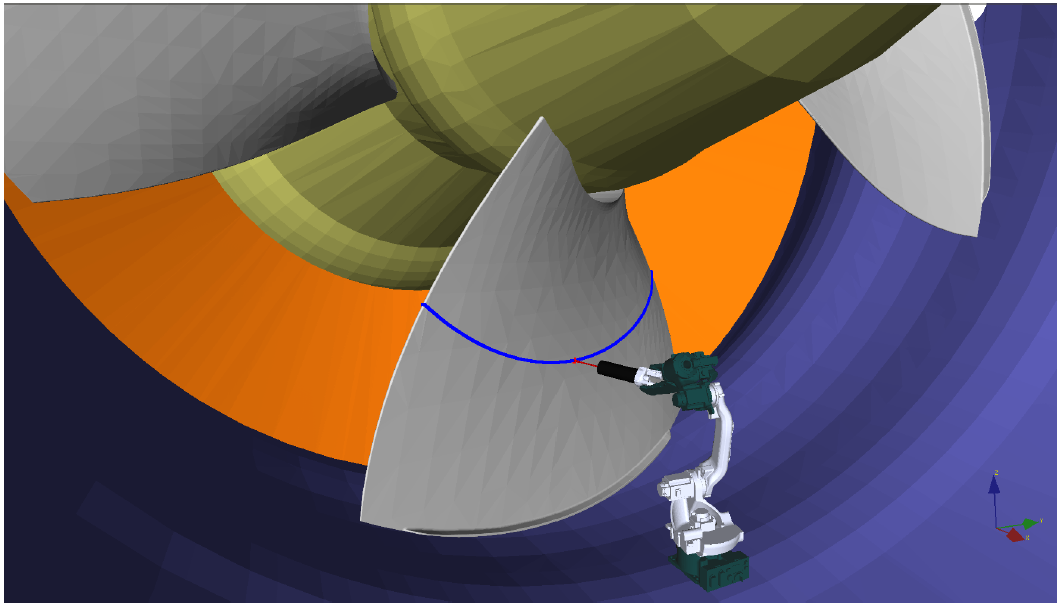
\includegraphics[width=0.75\textwidth]{figs/coat_blade}
 	\caption{Revestimento da face curva de uma pá. \\Fonte: \ldots}
 	\label{fig::trajec_600x30}
 	\todo[inline]{Incluir fonte da figura do Renan}
\end{figure}

As trajetórias para representar este processo serão simplificadas neste
trabalho, pela consideração de que as superfícies são planas e que pode-se
representar a trajetória totalmente naquele plano.

A trajetória será modelada pelo conjunto de funções das posições de referência
para cada coordenada generalizada. Como o planejamento é feito pela função da
posição da ferramenta no tempo, são utilizadas as soluções da cinemática
inversa, desenvolvidadas na seção~\ref{sec::ikin_mh12}.

É claro que dependendo da posição e orientação da superfície a ser coberta pelo
robô, este assumirá diferentes configurações, que causam excitações diferentes
em sua base. Na seção~\ref{sec::casos}, diversos casos de trajetória e bases
serão analisados, com o objetivo de verificar os efeitos também da trajetória
nos erros devido a dinâmica do sistema robô-base. 

Para exemplificar os conceitos abordados nesta seção, considere-se a seguinte
tarefa para cálculo da trajetória:
\newline
\begin{tcolorbox}
[colframe=black!75!white, colback=white, title = Trajetória -Exemplo] 
  \textbf{Tarefa:} Revestimento por HVOF \\
  \textbf{Área:} $(600 \times 300)~mm^2$ \\
  \textbf{Ponto inicial:} $\mathbf{p}_f = [0,700,~1,238,~-0,600]^Z$ \\
  \textbf{Orientação:} $\boldsymbol{\Phi}_{f} = [0,~0,~0]^Z$ \\
  \textbf{Passo:} $10~mm$ \\
  \textbf{Número de paralelos:} 50 \\
  \textbf{Velocidade da ferramenta:} $40~m/min$
\end{tcolorbox}
%
De acordo com o exemplo, a orientação do plano da superfície,
está alinhado ao sistema de coordenadas inercial e paralelo ao plano xz. A
Figura~\ref{fig::trajec_600x500x10} apresenta os 50 paralelos da trajetória ao
longo desta região.

\begin{figure}[h]
	\centering 
 	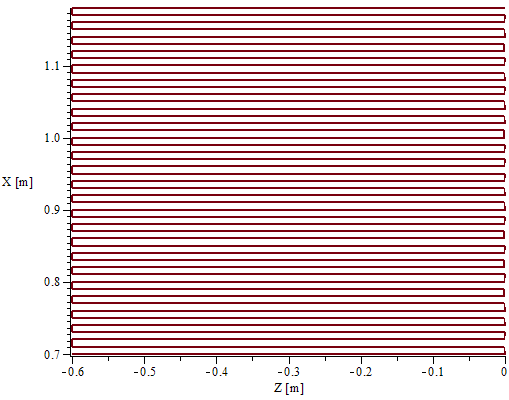
\includegraphics[width=0.70\textwidth]{figs/trajec_600x500x10}
 	\caption{Exemplo da trajetória de revestimento de uma região}
 	\label{fig::trajec_600x500x10}
\end{figure}

A Figura~\ref{fig::trajec3D_600x500x10} apresenta essa tarefa no ambiente 3D
de simulação, com o robô no início da trajetória. 

\begin{figure}[h!]
	\centering 
 	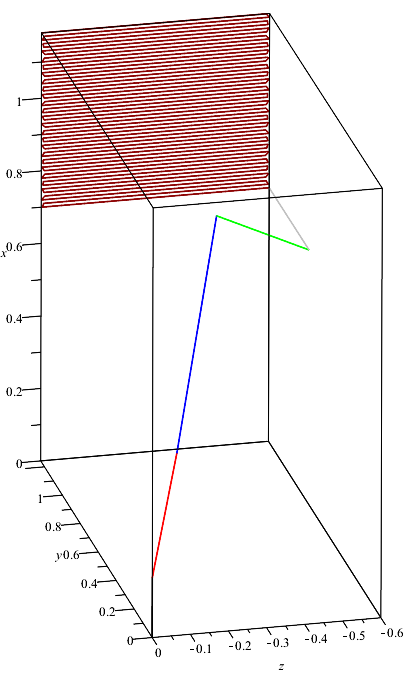
\includegraphics[width=0.50\textwidth]{figs/trajec3D_600x500x10}
 	\caption{Trajetória no ambiente 3D}
 	\label{fig::trajec3D_600x500x10}
\end{figure}

\subsubsection{Caminho ponto-a-ponto e função da trajetória}

O objetivo é determinar a função da trajetória em que robô realiza a tarefa de
revestimento. Primeiramente, define-se o conjunto ponto-a-ponto que forma o
caminho. A função temporal que liga os pontos do caminho é a trajetória.

Os pontos serão definidos nos vértices em que há mudança de direção da
ferramenta, ou seja, no início e fim de cada paralelo. Cada ponto será descrito
pela sua posição no ambiente em função do tempo. Logo:
%
\begin{equation} \label{eq::posi}
	\mathbf{p}_i = [~ px_{i}(t),~ py_{i}(t),~ pz_{i}(t)~]^Z
\end{equation}
%
Deseja-se que a velocidade da ferramenta entre os pontos seja controlada pelo
PID. Então, é preciso que a derivada da função trajetória entre os pontos seja a
velocidade desejada. Logo, a função da trajetória entre dois pontos de um mesmo
paralelo pode ser escrita como:
%
\begin{equation} \label{eq::pi}
\begin{split}
	p_i & = p_{i-1} + v \cdot \Delta t \\
		& = p_{i-1} + v \cdot (t-t_{i-1})
\end{split}
\end{equation}
%
Onde $v$ é a velocidade da ferramenta do ponto $p_{i-1}$ a $p_{i}$ e
$\Delta t$ é a variação de tempo entre o instante $t$ e o valor do tempo no
início da trajetória naquele paralelo $t_{i-1}$. A velocidade considerada neste
exemplo é de $40~m/min$.

Pode-se então calcular o intervalo de tempo entre cada ponto do caminho por:
%
\begin{equation} \label{eq::dt}
	\Delta t = \frac{p_i - p_{i-1}}{v}
\end{equation}
%
Portanto, o tempo associado a cada ponto do caminho é determinado por:
%
\begin{equation} \label{eq::ti}
	t_i = t_{i-1} + \Delta t
\end{equation}
%
Com as equações~\ref{eq::pi} e \ref{eq::ti}, define-se a função da trajetória
para cada paralelo.
%
\begin{table}[h]
\centering
\caption{Resumo dos pontos e funções trajetória do exemplo}
\label{tab::func_paralelos}
\begin{tabular}{|c|c|c|c|c||c|c|c|}
\hline
i & $px_i$ & $py_i$ & $pz_i$ & $t_i$  & $px_i(t)$    & $py_i(t)$ &
$pz_i(t)$
\\ \hline \hline
1       & 0,70  & 0,8   & -0,6  & 1,000 & 0,7         & 0,8      & -0,6         \\ \hline
2       & 0,70  & 0,8   & 0     & 1,900 & 0,7         & 0,8      & -1,27+0,67t  \\ \hline
3       & 0,71  & 0,8   & 0     & 1,915 & -0,57+0,67t & 0,8      & 0            \\ \hline
4       & 0,71  & 0,8   & -0,6  & 2,815 & 0           & 0,8      & 1,27-0,67t   \\ \hline
5       & 0,72  & 0,8   & -0,6  & 2,830 & -1.167+.67t & 0,8      & -0,6         \\ \hline
6       & 0,72  & 0,8   & 0     & 3,730 & 0,72        & 0,8      & -2,487+0,67t \\ \hline
7       & 0,73  & 0,8   & 0     & 3,745 & -1,77+0,67t & 0,8      & 0            \\ \hline
8       & 0,73  & 0,8   & -0,6  & 4,645 & 0,73        & 0,8      & 2,497-0,67t  \\ \hline
\end{tabular}
\end{table}
%

A Tabela~\ref{tab::func_paralelos} apresenta os termos do vetor posição da
equação~\ref{eq::posi} e as funções trajetória para os primeiros 4 paralelos do
exemplo. A Figura~\ref{fig::pontos_exemplo} ilustra os pontos indicados na
tabela no gráfico da trajetória.

\begin{figure}
	\centering 
 	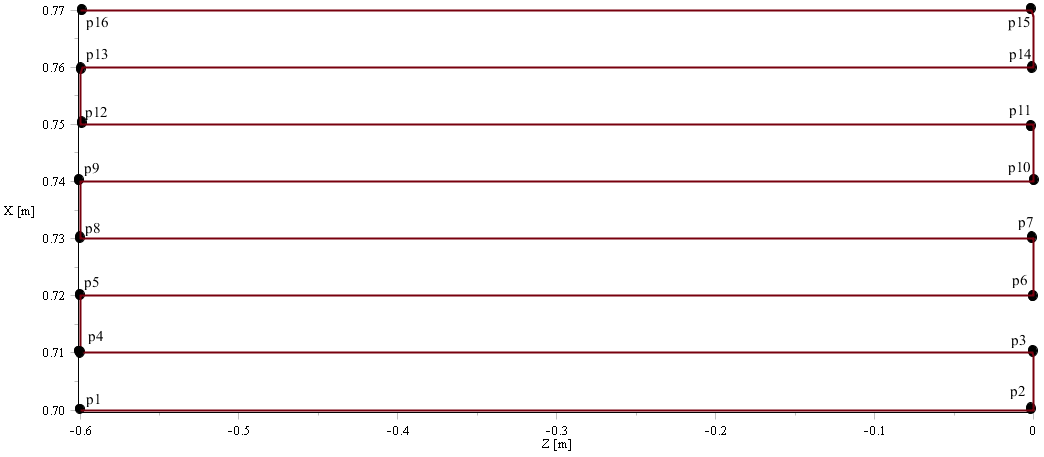
\includegraphics[width=0.90\textwidth]{figs/pontos_exemplo}
 	\caption{Os pontos do caminho dos 8 primeiros paralelos}
 	\label{fig::pontos_exemplo}
\end{figure}

\subsubsection{\textit{Piecewise function} e cinemática inversa}

As funções $px_i(t), py_i(t)$ e $pz_i(t)$, podem ser tratadas como uma única
função, através do uso do comando \texttt{piecewise}, no Maple. Os argumentos
deste comando são simplesmente as funções contidas em cada intervalo de tempo,
resultando em uma função única, dividida por partes, sem necessidade de serem
contínuas. A vantagem é que essas funções podem ser derivadas, sendo reconhecido
que na discontiuidade a função é indefinida.
Outra vantagem é que pode ser utilizada diretamente para calcular, por meio da
cinemática inversa, as funções das coordenadas generalizadas que descrevem o
conjunto de posições, para todo o intervalo de tempo.

No Maple, a função \textit{piecewise} resultante tem a seguinte forma:
%
\begin{equation}
p_{piecewise} = 
\begin{cases}
p0 & t<t1 \\
p1 & t<t2 \\
p2 & t<t3 \\
p3 & t<t4 \\
p4 & otherwise
\end{cases}
\end{equation}
%

Pelas equações~\ref{eq::q3ik} a \ref{eq::q6ik} foram definidas as coordenadas
generalizadas $q1$ a $q6$ em funcão da posição da ferramenta, $\mathbf{p}_f^Z$.
Logo, basta substituir a função \textit{piecewise} de cada termo de
$\mathbf{p}_f^Z$ em $q1$ a $q6$ para obter o resultado da cinemática inversa por
partes, ou intervalos de tempo.

Esta nova função será utilizada como parâmetro de entrada no modelo dinâmico,
para as coordenadas de referência $q_1ref$ a $q_5ref$. Isso faz com que o
controle PID forneça os torques para atingir estas coordenadas ao
longo do tempo e assim perseguir a trajetória determinada. A
Figura~\ref{fig::res_exemplo} apresenta o gráfico do resultado da cinemética
inversa utilizando as função \textit{piecewise} para a posição e velocidade da
ferramenta durante os primeiros 8 paralelos da tarefa. 

\begin{figure}[h]
    \centering
    \begin{subfigure}[b]{0.40\textwidth}
        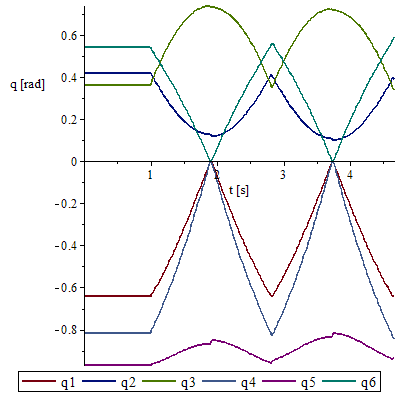
\includegraphics[width=\textwidth]{figs/qxt_exemplo}
        \caption{Resultado dos ângulos de referência}
        \label{fig::qxt_exemplo}
    \end{subfigure}
    \quad %add desired spacing between images, e. g. ~, \quad, \qquad, \hfill
    % etc.
      %(or a blank line to force the subfigure onto a new line)
    \begin{subfigure}[b]{0.4\textwidth}
        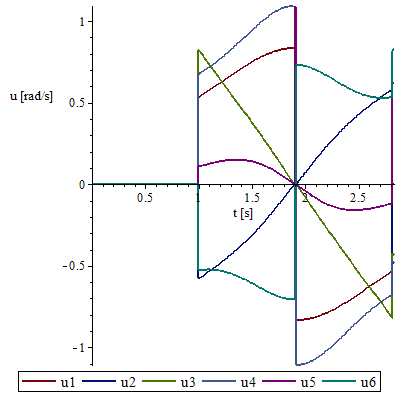
\includegraphics[width=\textwidth]{figs/uxt_exemplo}
        \caption{Resultado das velocidades de referência}
        \label{fig::uxt_exemplo}
    \end{subfigure}
    \caption{Resultados do exemplo de trajetória}\label{fig::res_exemplo}
\end{figure}


\subsection{Modelo teórico MBS -- Robô}

Nas seções anteriores foram desenvolvidas as equações simbólicas para a
cinemática direta, cinemática inversa e dinâmica do manipulador robótico.
Obteve-se portanto um moodelo para a Dinâmica Multicorpos (MBS) do robô, de tal
forma que é possível seguir uma lista de procedimentos e dados de entrada para
realizar simulações de qualquer tarefa que se desejar. Com o modelo MSB do robô,
os procedimentos para simular uma tarefa muito resumidamente são:

\begin{enumerate}
  \item Definir os sistemas de coordenadas de cada elo do robô;
  \item Definir as coordenadas generalizadas em cada junta;
  \item Fornecer os parâmetros de geometria e inércia do robô;
  \item Definir os parâmetros do controlador PID em cada junta;
  \item Definir a configuração inicial do robô;
  \item Fornecer os requisitos da tarefa (no caso do revestimento: plano,
  velocidade, passo, etc)
  \item Definir os pontos do caminho a ser percorrido pela ferramenta;
  \item Utilizar o resultado da trajetória como as coordenadas de referência no
  modelo dinâmico;
  \item Realizar a simulação da tarefa. 
\end{enumerate}

Utiliza-se novamente o exemplo abordado na seção~\ref{sec::tarefa_traj} para
demonstrar os resultados obtidos pelo modelo MBS. Dada portanto a tarefa de
revestimento do exemplo, realiza-se a simulação do modelo dinâmico com os
valores de referência para o PID fornecido pela cinemática inversa.

Os resultados serão apresentados para os primeiros 4 paralelos, a fim de
facilitar sua visualização. Este modelo MBS, desenvolvido no Maple, conta com
um resultado esquemático da animação do movimento do robô realizando a
trajetória. A região sendo coberta pelo revestimento é impressa na animação
durante o movimento. A sequência de Figuras~\ref{fig::mbs3D_exemplo} fornece uma
visulização simplificada da animação, ``fotografada'' em vários instantes de
tempo.

\begin{figure}[h]
    \centering
    \begin{subfigure}[b]{0.4\textwidth}
        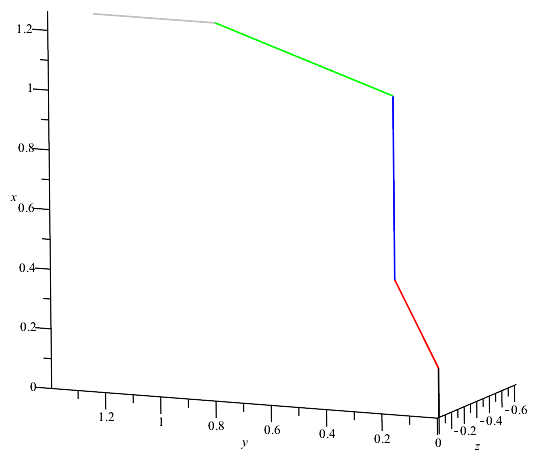
\includegraphics[width=\textwidth]{figs/mbs3D_0s}
        \caption{$0~s$}
        \label{fig::mbs3D_0s}
    \end{subfigure}
    \quad %add desired spacing between images, e. g. ~, \quad, \qquad, \hfill
    % etc.
      %(or a blank line to force the subfigure onto a new line)
    \begin{subfigure}[b]{0.4\textwidth}
        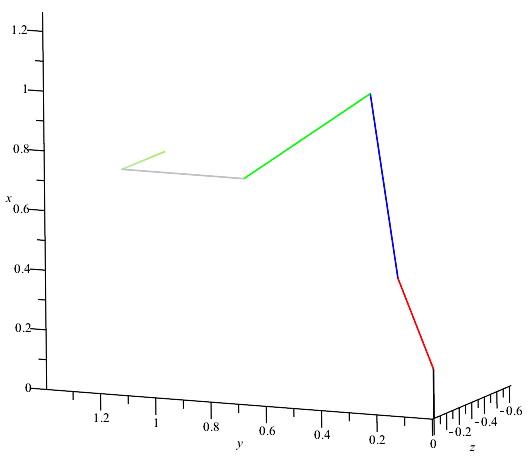
\includegraphics[width=\textwidth]{figs/mbs3D_1s5}
        \caption{$1,5~s$}
        \label{fig::mbs3D_1s5}
    \end{subfigure}
    \quad %add desired spacing between images, e. g. ~, \quad, \qquad, \hfill
    % etc.
      %(or a blank line to force the subfigure onto a new line)
    \begin{subfigure}[b]{0.4\textwidth}
        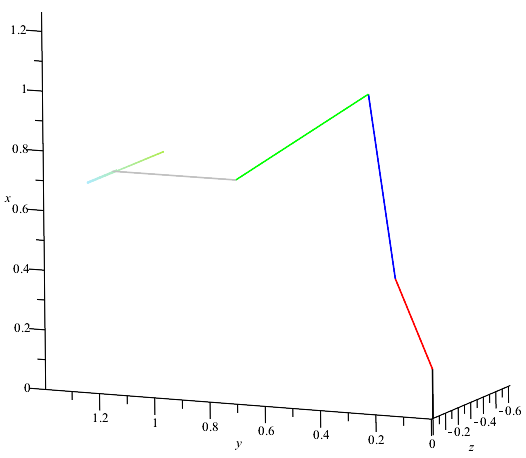
\includegraphics[width=\textwidth]{figs/mbs3D_2s5}
        \caption{$2,5~s$}
        \label{fig::mbs3D_2s5}
    \end{subfigure}
    \quad %add desired spacing between images, e. g. ~, \quad, \qquad, \hfill
    % etc.
      %(or a blank line to force the subfigure onto a new line)
    \begin{subfigure}[b]{0.4\textwidth}
        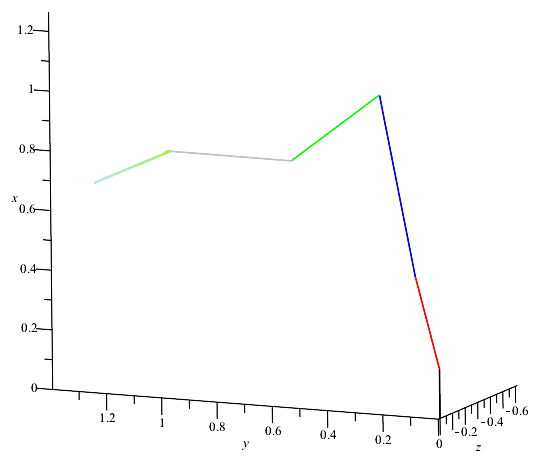
\includegraphics[width=\textwidth]{figs/mbs3D_3s}
        \caption{$3~s$}
        \label{fig::mbs3D_3s}
    \end{subfigure}
    \caption{Animação da trajetória no ambiente 3D} \label{fig::mbs3D_exemplo}
\end{figure}

O próximo resultado compara a variação angular das juntas ideal, pelo cálculo da
cinemática inversa, e o efetivo, resultado da trajetória no modelo dinâmico.
A Figura~\ref{fig::qxt_ex_realxideal} apresenta em linha pontilhada o valor dos
ângulos ideais, e em linha cheia, os efetivos.

\begin{figure}[h]
	\centering 
 	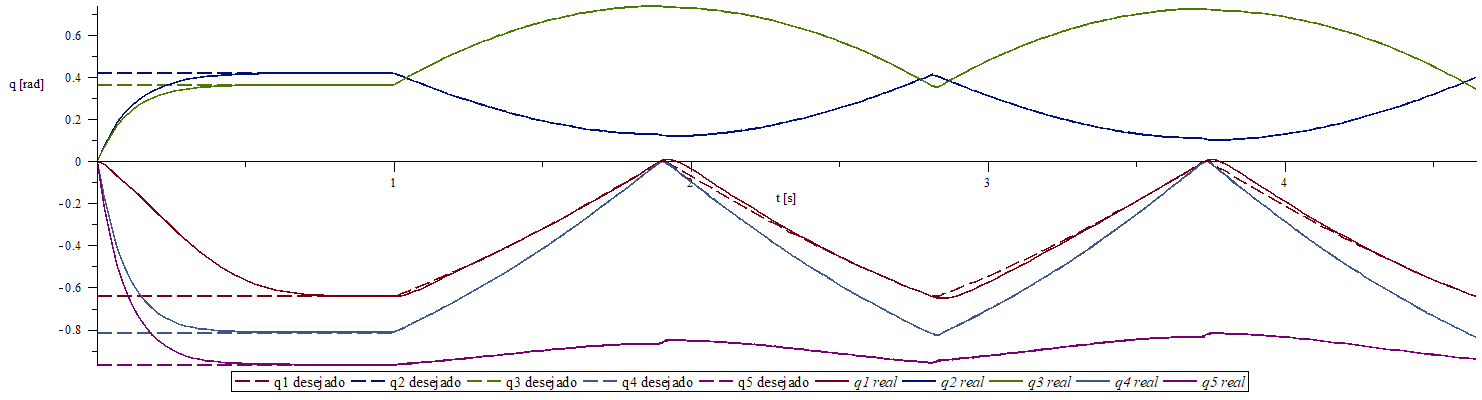
\includegraphics[width=0.95\textwidth]{figs/qxt_ex_realxideal}
 	\caption{Comparação ideal x efetivo dos ângulos das juntas}
 	\label{fig::qxt_ex_realxideal}
\end{figure}

Outro resultado analisado é a posição efetiva da ponta da ferramenta, em
comparação com a idealizada na cinemática inversa. Esse resultado será
extremamente importante para avaliar os casos de diferentes bases do modelo
acoplado robô-base e permitirá verificar o critério de erros máximos admissíveis
para o processo. A Figura~\ref{fig::errop_exemplo} apresenta o resultado
comparativo entre as posições ideais e efetivas. Cada linha do gráfico
representa uma coordenada (x, y, z) do vetor posição da ferramenta.

\begin{figure}[h]
	\centering 
 	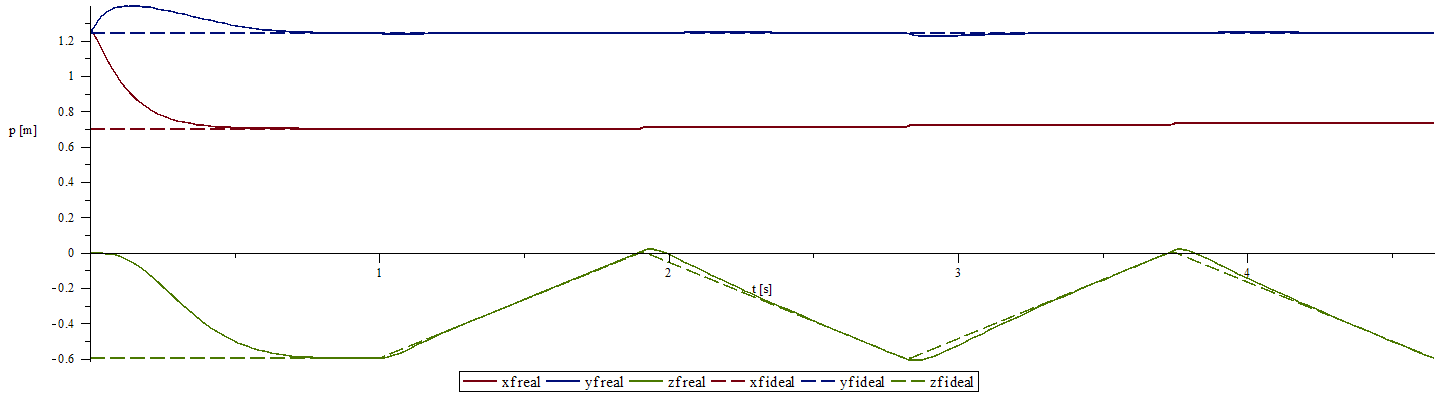
\includegraphics[width=0.95\textwidth]{figs/errop_exemplo}
 	\caption{Comparação ideal x efetivo da posição da ferramenta}
 	\label{fig::errop_exemplo}
\end{figure}

Nota-se que neste modelo MBS o robô é capaz de seguir com boa precisão a
trajetória informada. Para facilitar a visualização, a
Figura~\ref{fig::erros_exemplo} apresenta um gráfico do erro de cada coordenada
da posição, ao longo da trajetória. A linha pontilhada representa o erro
absoluto, ou seja, a norma do erro em cada direção.

\begin{figure}[h]
	\centering 
 	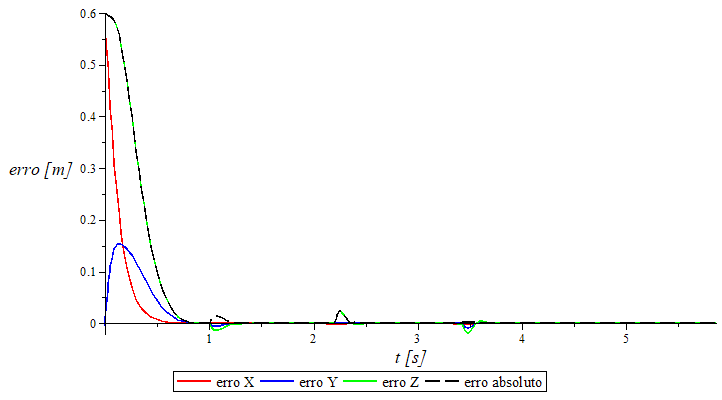
\includegraphics[width=0.95\textwidth]{figs/erros_exemplo}
 	\caption{Erro de posição da ferramante em cada direção}
 	\label{fig::erros_exemplo}
\end{figure}

Observa-se por este resultado que o erro de posicionamento, a partir do início
da região a ser revestida ($t>1s$), é da ordem de $10^{-1}~mm$ durante
apriximadamente $70\%$ do caminho de um paralelo. Próximo ao início e fim dos
paralelos, esse erro cresce, devido ao transitório de direção e sentido do
deslocamento, que não são acompanhados perfeitamente pela dinâmica do robô.
Estes erros chegam a uma ordem de $10~mm$ nestas regiões.

Da mesma forma que foi feito para a posição, pode-se verificar os erros de
velocidade da ferramenta. Para isso, deriva-se a a posição da ferramenta, com
respeito ao tempo e obtém-se o vetor velocidade. O resultado de cada componente
e do valor absoluto do erro para a tarefa do exemplo é apresentado na
Figura~\ref{fig::errovel_exemplo}.

\begin{figure}[h]
	\centering 
 	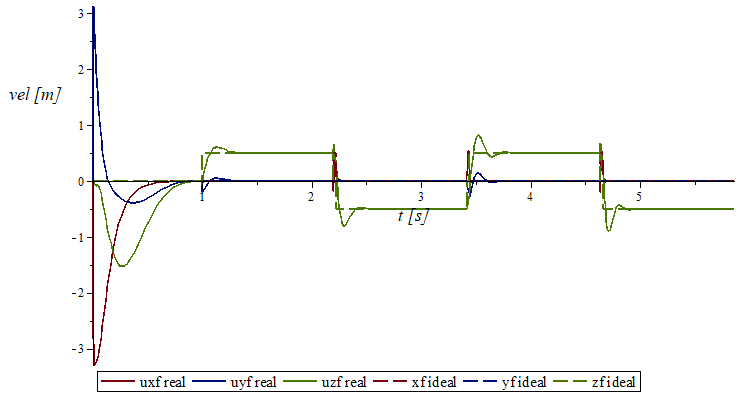
\includegraphics[width=0.95\textwidth]{figs/errovel_exemplo}
 	\caption{Erro de velocidade da ferramenta em cada direção}
 	\label{fig::errovel_exemplo}
\end{figure}

Os erros tolerados variam de acordo com os critérios definidos na
seção~\ref{sec::requisitos}\todo{Incluir seção com os requisitos do
revestimento} e serão analisados mais detalhadamente na
seção~\ref{sec::casos}.

Por último, calcula-se o erro de orientação, definido como a diferença
entre a orientação da superfície dada pela tarefa e obtida pela cinemática
inversa, e a orientação resultante da dinâmica.

É representada por uma matriz, determinada pela transformação homogênea entre o
referencial inercial, SC-Z, e o referencial localizado no pulso, SC-B, já que a
ferramenta é fixada neste último. Logo, pode-se comparar as duas matrizes, ideal
e efetiva, para cálculo do erro.

Uma maneira mais prática de representar o erro de orientação é por meio de um
escalar, que represente o ângulo de desvio da ferramenta entre o caso ideal e o
efetivo. Isto pode ser feito levando em consideração que estas matrizes são
formadas por vetores unitários dispostos nas colunas da matriz e formam uma
base ortonormal.\todo{Incluir teorema que calcula o angulo entre as bases}.

Seja a orientação ideal representada pela matriz $Mi$, que é função dos 3
ângulos de Euler $\phi,~\theta$ e $\psi$, e a matriz resultante da dinâmica por
$Me$, função do resultado de $q1(t),\ldots,q5(t)$, calcula-se:
%
\begin{equation}
	R = Me(q(t))~Mi(\phi,\theta,\psi)^{-1}
\end{equation}
%
Aplicando $R$ à equação~\ref{eq::angdesvio}, calcula-se o ângulo de desvio entre
as duas matrizes.
%
\begin{equation} \label{eq::angdesvio}
	\theta_{erro} = \arccos\left(\frac{tr(R)-1}{2}\right)
\end{equation}
%
Para a tarefa do exemplo, as matrizes $Me$ e $Mi$ e $R$ em, por exemplo,
$t=2~s$ são:
%
 \begin{gather*}
 % eq1
 Me = \left[ \begin {array}{ccc}  0.99755& 0.0&- 0.069955
\\ \noalign{\medskip}- 0.00262& 0.99930&- 0.037325
\\ \noalign{\medskip} 0.069903& 0.037413& 0.99685\end {array} \right] \\
% eq2
 Mi =  \left[ \begin {array}{ccc}  1~& 0~& 0~\\ \noalign{\medskip} 0~&
 1~& 0~\\ \noalign{\medskip} 0~& 0~& 1~\end {array} \right] \\
 % eq3
R =  \left[ \begin {array}{ccc}  1.0&- 0.00000058757&- 0.0021389
\\ \noalign{\medskip}- 0.000079441& 0.99930&- 0.037415
\\ \noalign{\medskip} 0.0021374& 0.037415& 0.99930\end {array}
 \right]
\end{gather*}
%
Aplicando $R$ na equação~\ref{eq::angdesvio}, obtém-se o erro de orientação
neste instante de tempo.
%
\begin{equation*}
	\theta_{erro}(t=2~s) = 0.0374898~rad
\end{equation*}
%
O resultado do desvio de orientação da ferramenta, ao longo de toda a tarefa é
apresentado no gráfico da Figura~\ref{fig::orierro_exemplo}.

\begin{figure}[h]
	\centering 
 	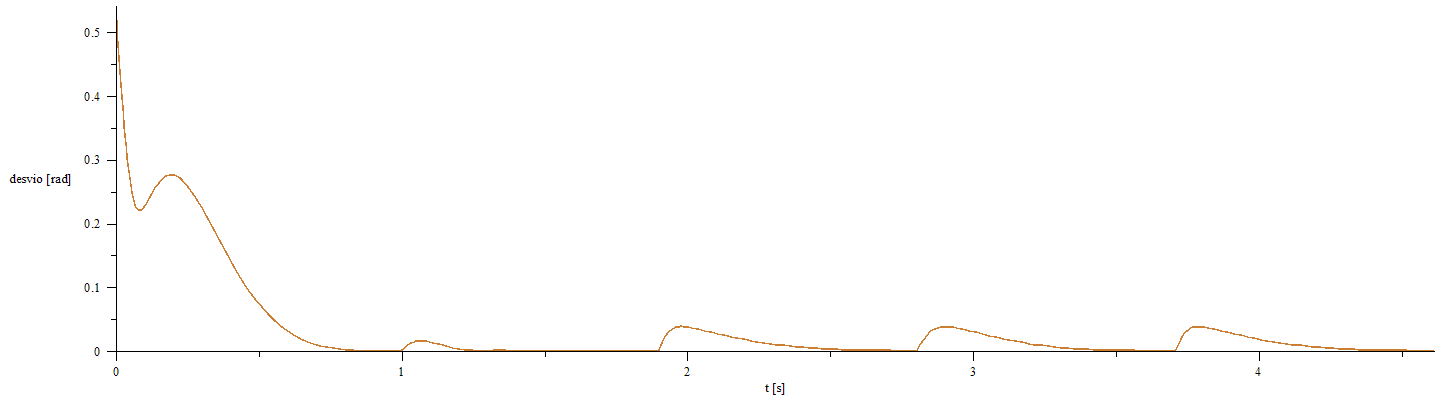
\includegraphics[width=0.95\textwidth]{figs/orierro_exemplo}
 	\caption{Erro de orientação da ferramenta}
 	\label{fig::orierro_exemplo}
\end{figure}

Novamente, nesta tarefa do exemplo, não se está interessado no erro antes do
manipulador iniciar a trajetória dos paralelos do revestimento, ou seja, entre a
posição inicial e o ponto p1.
Analisando, portanto, o gráfico a partir de $1~s$ percebe-se um erro periódico,
maior devido às variações de direção, com amplitude máxima de aproximadamente
$0,038~rad$, ou $2,18^{\circ}$.

Apesar de não ser possível, apenas por este resultado escalar, afirmar a direção
onde o erro é maior, pode-se comparar com o gráfico do erro de posicionamento,
na Figura~\ref{fig::erros_exemplo}. É possível inferir que este erro está mais
relacionado com o atraso do posicionamento na direção $z$ e portanto, grande
parte do desvio de orientação está na direção vertical, $x$ de SC-Z.

Nesta seção foram explorados os resultados que simulações utilizando o modelo
MBS podem fornecer. Para isso, tomou-se como exemplo uma tarefa de cobertura de
uma superfície plana. Os métodos de cálculo dos erros de posicionamento,
velocidade e orientação da extremidade da ferramenta foram demonstrados e serão
utilizados para comparação de diferentes casos do modelo acoplado robô-base
flexível, realizando tarefas de revestimento de superfícies planas, que serão
propostos na seção~\ref{sec::casos}.






% -.~.-.~.-.~.-.~.-.~.-.~.-.~.-.~.-.~.-.~.-.~.-
\section{Modelo da base} \label{sec::base}

A base é definida, neste trabalho, como qualquer estrutura, à qual o manipulador
robótico é fixado, que forneça flexibilidade, em forma de graus de liberdade,
passivos das forças dinâmicas exercidas pelo movimento do robô. A flexibilidade
da estrutura causará desvios do movimento esperado e controlado do robô e cabe
ao método proposto tentar quantificar esses desvios e verificar se os requisitos
do processo serão satisfeitos. Para isso, é desenvolvido um modelo teórico da
base, para ser adicionado ao modelo do robô, formando um sistema MBS acoplado.

Nesta seção é demonstrado como uma estrutura construída com geometria,
materiais, restrições e infinitos graus de liberdade que seriam muito complexos
para serem descritos analiticamente em um modelo MBS, pode ser simplificado como
um sistema de massa-mola-amortecedor de 6 graus de liberdade.
Considera-se um conjunto de sistemas de coordenadas localizado no ponto teórico
onde é fixado o robô, na estrutura. A esse sistema, correspondem 3 movimentos de
translação $x,y,z$ e 3 movimentos de rotação $\theta_x, \theta_y, \theta_z$, que
formam as coordenadas generalizadas do modelo MBS.

Portanto, para realizar a simplificação é necessário obter uma matriz de rigidez
e uma matriz de amortecimento, associadas aos 6 gdl do corpo sobre a base. A
matriz de rigidez é obtida numericamente pela Análise por Elementos Finitos
(AEF) e a matriz de amortecimento pelo resultado experimental do ensaio de
vibrações seguido do tratamento dos resultados, detalhado na
seção~\ref{sec::experimento}.

Por fim é demonstrado como são desenvolvidas as equações que regem o
movimento do corpo acoplado a esse sistema massa-mola-amortecedor.
Foi utilizada a mesma metodologia do modelo do robô para desenvolvimento das
equações de movimento: pelo método de Kane e com uso das rotinas do programa
Sophia-Maple.

\subsection{Geometria e CAD}

A primeira etapa para modelagem da base é representar sua geometria em um modelo
CAD. Este modelo será utilizado para as simulações pela Análise por Elementos
Finitos, a fim de se obter a sua matriz de rigidez.

Para ilustrar o método, será aproveitada a base projetada e construída para
testes do robô, em laboratório, previstos no projeto EMMA. Consiste em uma
estrutura metálica, formada por perfis extrudados de alumínio estrutural. Sobre
a estrutura um par de trilhos paralelos permitem o movimento longitudinal da
placa onde é fixado o robô. A Figura~\ref{fig::estrut_modelo_fisico} apresenta
uma fotografia da base de testes.

\begin{figure}[h]
	\centering 
 	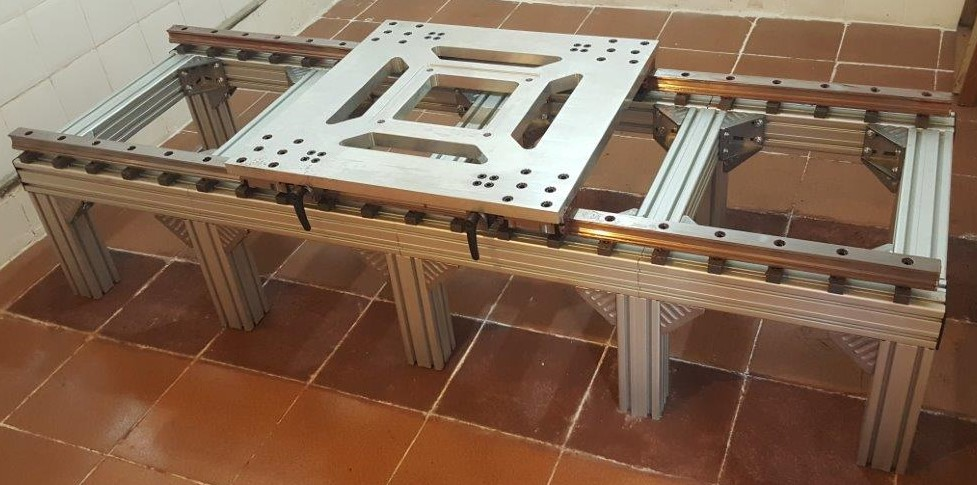
\includegraphics[width=0.70\textwidth]{figs/estrut_modelo_fisico}
 	\caption{Base de testes do robô}
 	\label{fig::estrut_modelo_fisico}
\end{figure}

O projeto desta base foi desenvolvido no programa SolidWorks, onde de forma
bastante detalhada, são incluídos os desenhos das peças customizadas, peças
comerciais, acessórios de união e fixadores mecânicos que compõe a montagem CAD
da estrutura. Este modelo é apresentado na Figura~\ref{fig::estrutCAD}, com os
principais componentes indicados, inclusive o robô.

\begin{figure}[h]
	\centering 
 	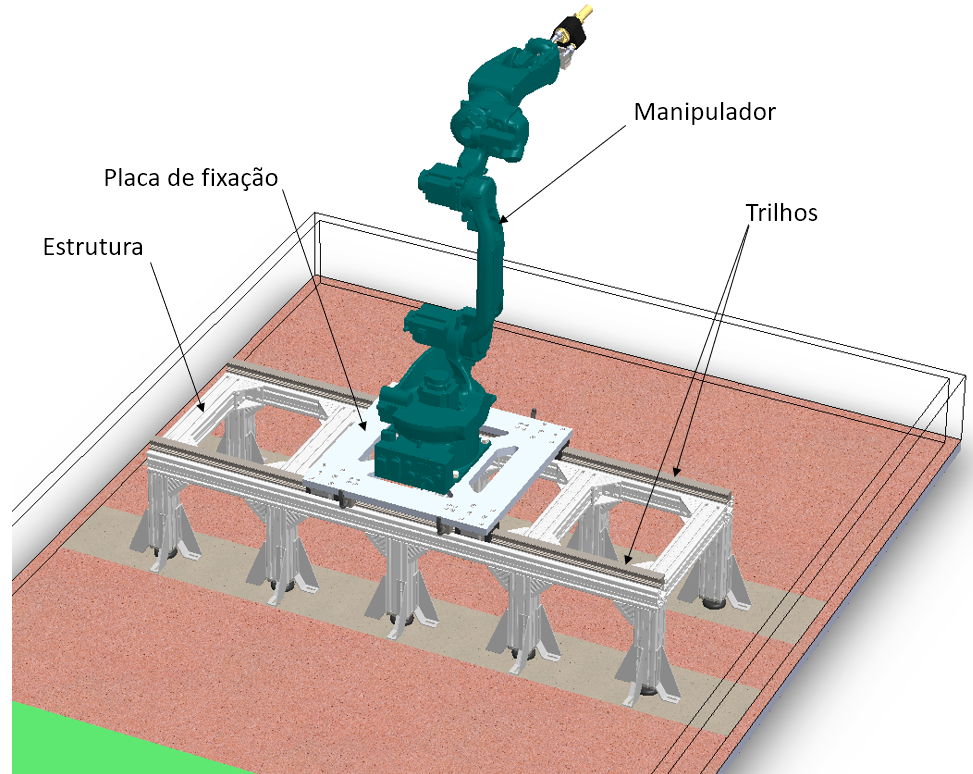
\includegraphics[width=0.75\textwidth]{figs/estrutCAD}
 	\caption{Modelo CAD detalhado da base e robô}
 	\label{fig::estrutCAD}
\end{figure}

Este modelo CAD, muito completo, poderia ser diretamente utilizado nas
simulações para obtenção da matriz de rigidez desta estrutura. No entanto, o
alto nível de detalhamento dos componentes, além da definição dos contatos e
restrições entre as peças, geraria um modelo de malha muito densa, não linear e
grande custo computacional. E o resultado teria muito informações irrelevantes
para esta análise, como por exemplo, tensões em elementos de fixação ou
deformação do rolamento do trilho.

Logo, o objetivo da simplificação é obter apenas os resultados que importam
na análise, e ignorar outros efeitos que não alteram significativamente
estes resultados. 

Para o modelo da base de testes, foram utilizados elementos unidimensionais, de
viga, para formar a estrutura e os trilhos. A união entre esses componentes foi
feita por elementos rígidos, representando os parafusos de fixação do trilho na
estrutura. A placa de fixação do robô foi representada também por elementos
unidimensionais rígidos, assumindo-se que sua rigidez é muito superior a rigidez
da estrutura, e o ponto de fixação do robô está localizado no centro desta
placa.
Os rolamentos do trilho foram substituídos por uma conexão rígida entre a placa
e os trilhos. Assim, a flexibilidade desta estrutura, no modelo simplificado
depende apenas das deformações dos elementos de viga que representam o trilho e
a estrutura. A Figura~\ref{fig::estrutFEA} apresenta o modelo simplificado para
a AEF, desenvolvida no programa Autodesk Simulation Mechanical.

\begin{figure}[h]
	\centering 
 	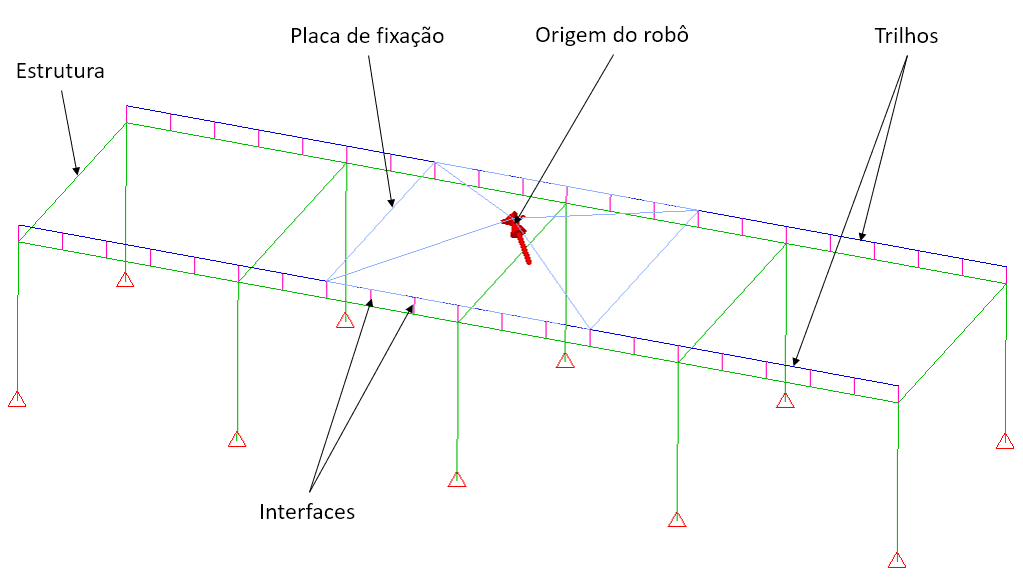
\includegraphics[width=0.75\textwidth]{figs/estrutFEA}
 	\caption{Modelo da base para AEF}
 	\label{fig::estrutFEA}
\end{figure}

\subsection{Análise por Elementos Finitos}

Foi demonstrado na seção~\ref{sec::rigidez} um método analítico e sistemático
para obter a matriz de rigidez de uma estrutura em qualquer ponto de
interesse. Para estruturas simples, com poucos graus de liberdade e poucos
elementos, o método analítico se mostra bastante prático. Já para estruturas
mais complexas, com muitos elementos, conexões, restrições, graus de liberdade
e não linearidades, resolver pelo método analítico pode ser impraticável ou
desgastante.

Como deseja-se a rigidez da estrutura para apenas um ponto de interesse -- o
ponto onde virtualmente está fixado o robô -- propõe-se uma forma de, utilizando
os conceitos do método apresentado e simulações por AEF, extrair a matriz de
rigidez para este ponto. As simulações realizadas são do tipo lineares e
estáticas. A seguir são detalhadas as etapas para definir o modelo para AEF.

\subsubsection{Partes, elementos e propriedades}

O modelo é divido em estrutura, trilho, interfaces e placa, como foi ilustrado
na Figura~\ref{fig::estrutFEA} Para cada parte são definidos o tipo de elemento,
suas propriedades e material.

A estrutura é formada por perfis de alumínio estrutural. Esta é modelada como
elementos unidimensionais de viga. Isso significa que suas propriedades são
uniformes ao longo de apenas uma dimensão em todo o elemento, bastando fornecer
apenas suas propriedades de seção transversal. A
Figura~\ref{fig::sectrans_bosch} mostra o corte de seção de um elemento da
estrutura e suas propriedades. O material associado à estrutura é o Alumínio
EN-AW-6060. e as propriedades são incluidas no modelo, de acordo com a
Tabela~\ref{tab::prop_mat}.

\begin{figure}[h]
	\centering 
 	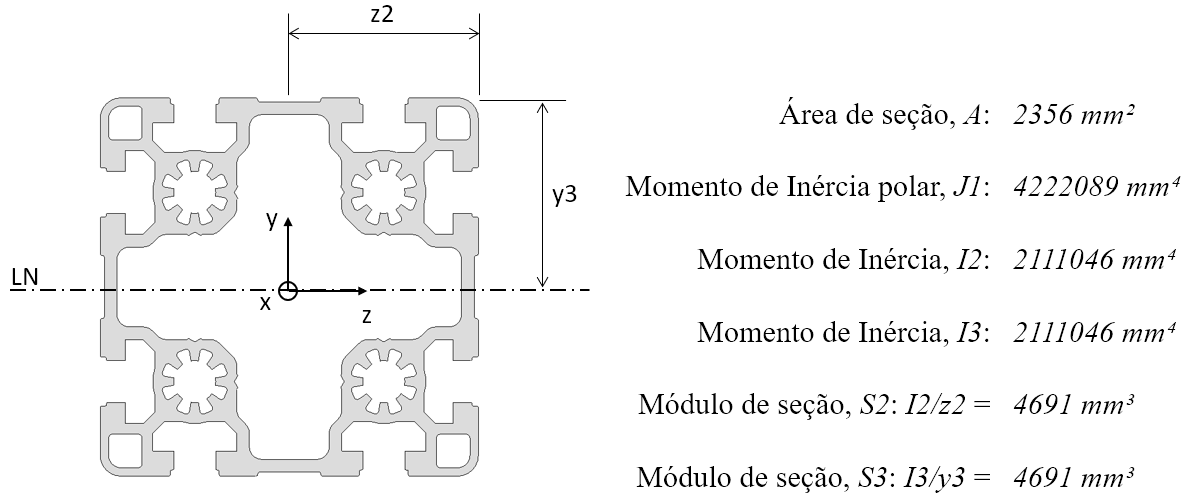
\includegraphics[width=0.85\textwidth]{figs/sectrans_bosch}
 	\caption{Seção transversal do elemento da estrutura}
 	\label{fig::sectrans_bosch}
\end{figure}

\begin{table}
\centering
\caption{Propriedades mecânicas dos materiais do modelo AEF}
\label{tab::prop_mat}
\begin{tabular}{@{}llcc@{}}
\toprule
\textbf{Propriedade}   &             & \textbf{EN-AW 6060} & \textbf{AISI 316} \\ \midrule
Densidade              & {[}g/cc{]}  & 2,70                & 7,90             \\
Módulo de Elasticidade & {[}GPa{]}   & 69,5                & 200               \\
Coeficiente de Poisson & {[}1{]}     & 0,34                & 0,29    			\\
Tensão de escoamento   & {[}MPa{]}   & 150                 & 240               \\
Resistência à tração   & {[}MPa{]}   & 150                 & 580               \\ \bottomrule
\end{tabular}
\end{table}

O trilho também é modelado como elemento de viga. Sua seção transversal e
propriedades estão na Figura~\ref{fig::sectran_trilho}. Seu material é o aço
carbono inoxidável AISI 316 e suas propriedades mecânicas estão na
Tabela~\ref{tab::prop_mat}.

\begin{figure}[h]
	\centering 
 	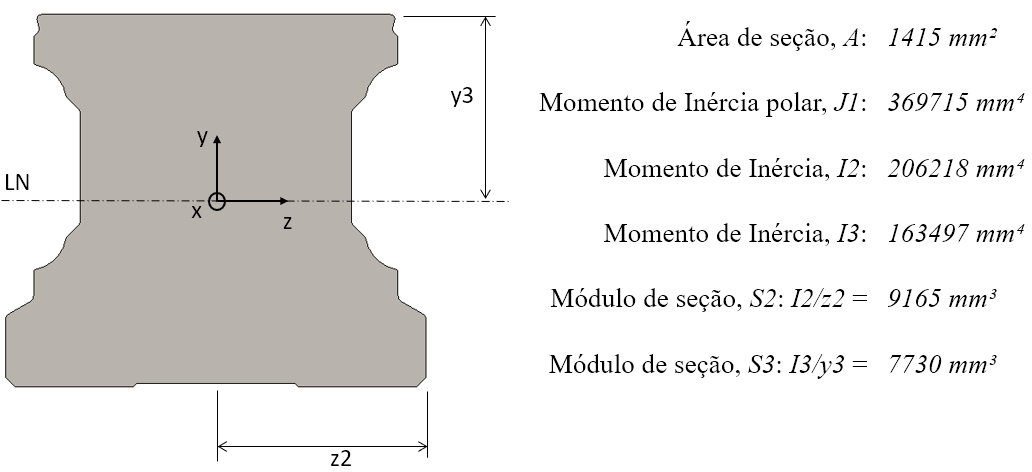
\includegraphics[width=0.85\textwidth]{figs/sectran_trilho}
 	\caption{Seção transversal do elemento do trilho}
 	\label{fig::sectran_trilho}
\end{figure}

As partes interface e placa de fixação do robô são modelados como elementos
unidimensionais rígidos, ou seja, transmitem apenas forças e momentos, mas não
se deformam. Ao todo são 40 peças de interface representando os 20 parafusos de
fixação de cada trilho. Já a placa de fixação é formada por um quadro de
elementos ligando os dois trilhos e uma ``pirâmide'' convergindo para o ponto de
fixação do robô. Como este ponto representa a conexão entre a estrutura e o
robô, aplica-se os esforços na estrutura diretamente por ali. Os elementos
rígidos transmitem estes esforços ao trilho e à estrtura e obtém-se os resultado
de forças de reação ou deslocamentos resultantes.


\subsubsection{Restrições e conexões}

Esta base é originalmente fixa no piso por meio de parafusos chumbadores. Cada
perna da estrurura posssui 3 parafusos. No modelo AEF, esta restrição será
modelada como fixa, ou seja, não permite-se nenhuma translação ou rotação, e
é aplicada à extremidade inferior de cada perna.

Os elementos de cada parte são conectados por uniões ``soldadas'', ou seja, não
permitem nenhum grau de liberdade na extremidade do elemento onde há a conexão.


\subsubsection{Casos de Carregamento}

Para obter a matriz de rigidez, deve-se realizar ao todo 6 casos de carregamento
e restrições. Cada caso obtém 6 dos 36 termos, que correspondem a uma linha
da matriz 6x6. Os carregamentos e restrições são todos aplicados ao ponto de
fixação do robô.

A cada caso será aplicado um deslocamento prescrito unitário em uma direção. Às
outras direções é aplicada restrição à translação e à rotação. Logo, um
deslocamento unitário na direção $x$ ($ux = 1~mm$), por exemplo, provoca uma
força ou momento de reação em todas as direções. A força de reação
correspondente à direção x produz o termo de rigidez $k_{11}$, à direção y, $k_{12}$,
à direção z, $k_{13}$, e assim por diante.

A Tabela~\ref{tab::casoscarreg} resume os casos e restrições
simulados.

\begin{table}[h]
\centering
\caption{Resumo dos casos de carregamento e restrições}
\label{tab::casoscarreg}
\begin{tabular}{@{}ccccccc@{}}
\toprule
\textbf{Caso} & \textbf{ux} & \textbf{uy} & \textbf{uz} & \textbf{rx} & \textbf{ry} & \textbf{rz} \\ \midrule
\textbf{1}    & $0,1~mm$           & fixo        & fixo        & fixo        &
fixo & fixo        \\
\textbf{2}    & fixo        & $0,1~mm$            & fixo        & fixo        &
fixo        & fixo        \\
\textbf{3}    & fixo        & fixo        & $0,1~mm$            & fixo        &
fixo        & fixo        \\
\textbf{4}    & fixo        & fixo        & fixo        & $0,001~rad$           
& fixo        & fixo        \\
\textbf{5}    & fixo        & fixo        & fixo        & fixo        &
$0,001~rad$            & fixo        \\
\textbf{6}    & fixo        & fixo        & fixo        & fixo        & fixo    
& $0,001~rad$            \\ \bottomrule
\end{tabular}
\end{table}


\subsubsection{Malha}

Os elementos do trilho e da estrutura foram subdivididos para gerar a malha. A
malha controla a qualidade do modelo e precisão do resultado.
Quanto menor o elemento, ou mais discretizada a malha, menor são os erros
numéricos da solução. O processo de refinamento da malha, consiste em realizar
simulações iterativamente, com malha cada vez mais discretizada. A comparação
dos resultados a cada iteração permite julgar uma convergência da solução. Logo,
é realizado este procedimento,, até que a diferença do resultado seja
insignificante.

O resultado deste processo de refinamento gerou a seguinte malha:
%
$$ 49~parts,~ 620~nodes,~ 670~elements $$
%

\subsubsection{Resultados por AEF}

Os resultados obtidos pela análise estática são a distribuição de tensões,
deslocamentos, forças e momentos de reação em cada nó do modelo. Um exemplo do
resultado de tensões e deslocamentos é apresentado na Figura~\ref{fig::res_FEA},
para o caso de carregamento 6.

\begin{figure}[h]
    \centering
    \begin{subfigure}[b]{0.8\textwidth}
        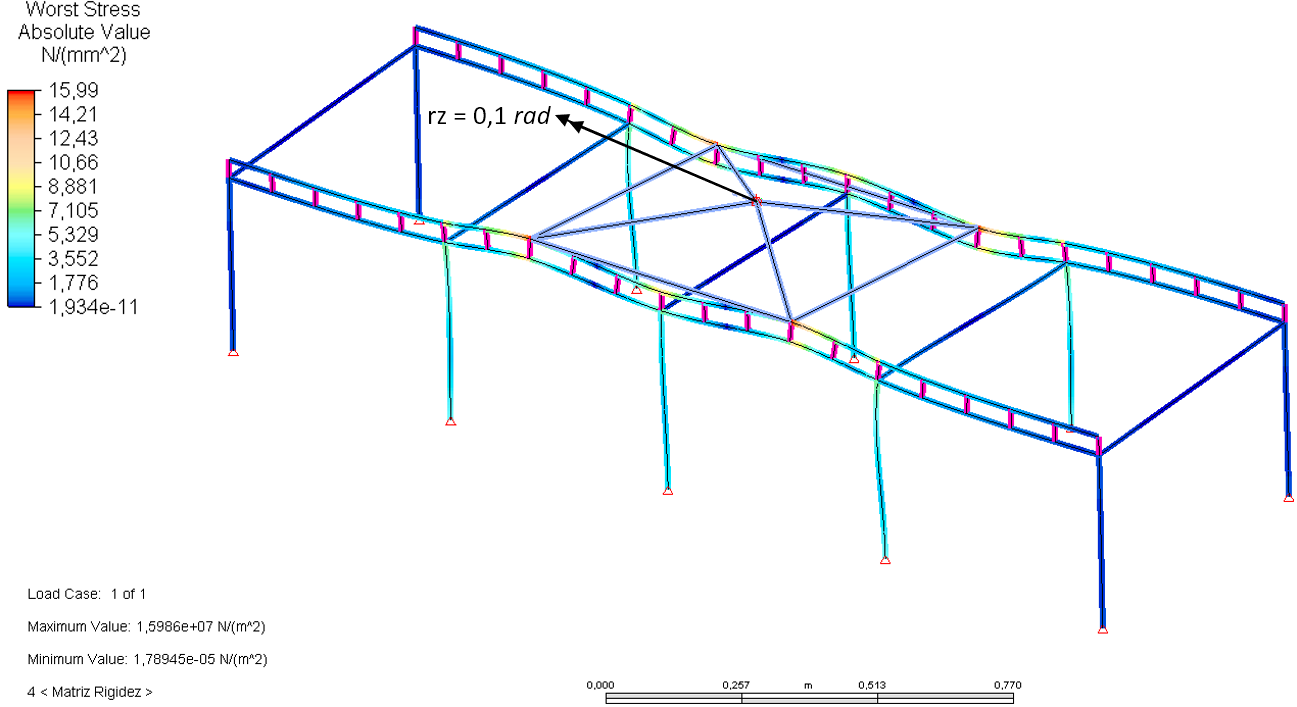
\includegraphics[width=\textwidth]{figs/res_FEA_tensoes}
        \caption{Resultado AEF das tensões máximas resultantes}
        \label{fig::res_FEA_tensoes}
    \end{subfigure}
    \quad %add desired spacing between images, e. g. ~, \quad, \qquad, \hfill
    % etc.
      %(or a blank line to force the subfigure onto a new line)
    \begin{subfigure}[b]{0.8\textwidth}
        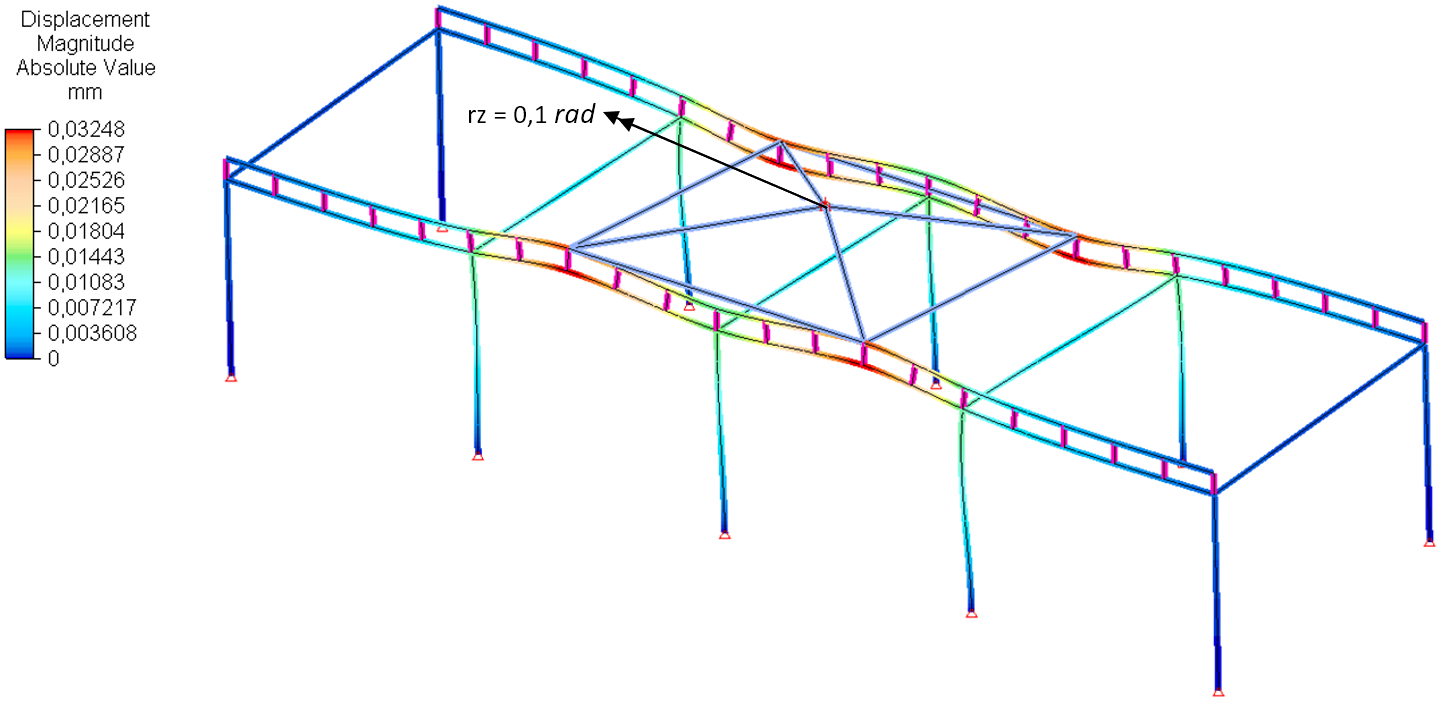
\includegraphics[width=\textwidth]{figs/res_FEA_desloc}
        \caption{Resultado AEF dos deslocamentos resultantes}
        \label{fig::res_FEA_desloc}
    \end{subfigure}
    \caption{Resultado da simulação AEF para o caso 6}
    \label{fig::res_FEA}
\end{figure}

O resultado das forças e momentos de reação no ponto de fixação do robô é
apresentado na Tabela~\ref{tab::res_FEA_forcas}. 

\begin{table}[h!]
\centering
\caption{Resultado das forças e momentos de reação para o caso 6}
\label{tab::res_FEA_forcas}
\begin{tabular}{@{}ccccccc@{}}
\toprule
\textbf{Caso} & \textbf{Fx [N]} & \textbf{Fy [N]} & \textbf{Fz [N]} &
\textbf{Mx [Nm]} & \textbf{My [Nm]} & \textbf{Mz [Nm]} \\ \midrule \textbf{6}   
& -3,00E-6 & 2,50E+3    & 1,67E-7    & 1,12E-6    & -7,16E-7   & -9,76E+3   \\ \bottomrule
\end{tabular}
\end{table}


\subsection{Matriz de Rigidez}

Deseja-se que a base seja simplificada como um sistema massa-mola-amortecedor de
6 gdl e introduzida no modelo MBS como uma matriz 6x6, que promove deslocamentos
ao robô, em função do carregamento resultante dos seus movimentos.

A matriz de rigidez possui 36 termos, chamados de coeficientes de influência.
A nomenclatura e posição de cada termo na matriz, está relacionado à direção da
força ou momento aplicado. Assim, o termo $k_{32}$ por exemplo refere-se a
rigidez na direção $y$, devido a uma força na direção $z$.

A matriz de rigidez tem a seguinte forma:
\begin{equation}
K = \begin{pmatrix} 
    k_{11} & \dots 	& k_{16} \\
    \vdots & \ddots & \\
    k_{61} &        & k_{66} 
    \end{pmatrix}
\end{equation}
%
Com o resultado das análises por AEF de cada caso, pode-se então calcular termo
a termo da matriz de rigidez da base. Como os deslocamentos prescritos são
arbitrários, faz-se o seguinte cálculo para converter a força de reação no
coeficiente de influência da matriz de rigidez:
%
\begin{align} \label{eq::kij}
	k_{ij} = \frac{F_j}{u_{i}} \qquad &  i,j = 1,\ldots,6
\end{align}
%
Onde $u_i$ representa o valor do deslocamento prescrito e $F_j$ o valor da força
ou momento de reação em cada caso de carregamento. A equação~\ref{eq::kij}
normaliza, portanto, o coeficiente de influência para um valor unitário de
deslocamento.

Note-se que, por definição, a matriz de rigidez é sempre positiva
definida\todo{Incluir referência para esta citação}, ou seja, simétrica e com
todos os autovalores positivos.
Isso faz com que não seja necessário calcular todos os 36 coeficientes de influências, mas apenas 21. 

Utilizando os resultados das simulações AEF e a equação~\ref{eq::kij}, a matriz
de rigidez para a base de testes é:
%
\begin{equation*}
	K =
\begin{pmatrix}
941490000 &	0 &	0 &	0 &	0 &	0 \\
0 &	130542000 &	0 &	0 &	0 &	-24981000 \\
0 &	0 &	262146000 &	0 &	5756560 &	0 \\
0 &	0 &	0 &	57018800 &	0 &	0 \\
0 &	0 &	5756560 &	0 &	119555000 &	0 \\
0 &	-24981000 &	0 &	0 &	0 &	97590600
\end{pmatrix}
\end{equation*}
%
A unidade dos valores da matriz estão convertidos para $[N/m]$. Os termos que
aparecem zerados não são exatamente zero, mas valores menores que 1 e, por
simplificação, foram considerados nulos.


\subsection{Matriz de Amortecimento}

O amortecimento será modelado como proporcional, ou de Rayleigh, como foi
explicado na seção~\ref{sec::amortecimento}. A matriz de amortecimento é
definida, pela equação~\ref{eq::amort_prop}, repetida a seguir:
%
\begin{equation*}
	C = \alpha M + \beta K
\end{equation*}
%
Logo, para definir totalmente a matriz de amortecimento da base, basta fornecer
os dois parâmetros, $\alpha$ e $\beta$.

Na seção~\ref{sec::param_mod} apresentou-se um método para, a partir dos dados
experimentais de amortecimento modal, obter os parâmetros $\alpha$ e $\beta$ que
melhor se ajustam ao modelo. Na seção~\ref{sec::experimento} é detalhado o
procedimento para se obter os valores experimentais de amortecimento e, a partir
do resultado, são calculados os parâmetros para obter a matriz de amortecimento.



\subsection{Modelo teórico MBS -- Base}

Equivalentemente ao realizado para o robô, a base será modelada como um
sistema dinâmico, cujas equações de movimento são desenvolvidas pelo método de
Kane.

O Sophia-Maple é novamente utilizado desde a construção do modelo cinemático até
a determinação das equações de movimento, exatamente como foi realizado o modelo
do robô. Como já foram apresentados os comandos e sintaxe do programa na
seção~\ref{sec::dkin}, não será repetido nesta seção, ciente de que os comandos
são equivalentes. No Anexo~\todo{Incluir código anexo} é fornecido o código
completo do modelo.

Para se chegar às equações de movimento, primeiramente, define-se os sistemas de
coordenadas e as coordenadas generalizadas do sistema.
As variáveis $q1, q2$ e $q3$ representam as 3 translações do ponto de fixação do
manipulador, em $x,y$ e $z$, respectivamente, em relação ao sistema de
coordenadas inercial, SC-R. As 3 rotações serão representadas pelas variáveis
$q4, q5$ e $q6$ e serão descritos nos sistemas de coordenadas SC-R1, SC-R2,
SC-R3, respectivamente.
A coordenada $q4$ representa um ângulo de rotacão do sistema de referência SC-R1
em relação ao sistema SC-R; $q5$ o ângulo entre SC-R2 e SC-R1; e $q6$ o ângulo
entre SC-R3 e SC-R2, formando uma cadeia cinemática de ângulos relativos. A
Figura~\ref{fig::schem_scbase} ilustra o sistema inercial SC-R e o sistema SC-R3
acoplado ao corpo sobre a base.

\begin{figure}[h]
	\centering 
 	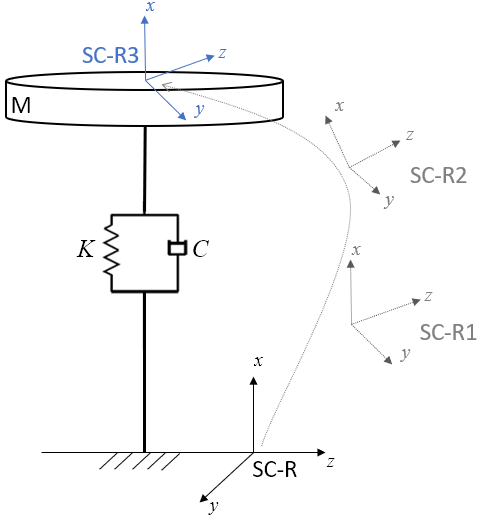
\includegraphics[width=0.5\textwidth]{figs/schem_scbase}
 	\caption{Desenho esquemático dos sistemas de referência da base e inercial}
 	\label{fig::schem_scbase}
\end{figure}

Neste modelo é considerado apenas um corpo, descrito em SC-R e localizado pelo
vetor $\mathbf{p}^M$, função de $q1,q2$ e $q3$.
%
\begin{equation}
	\mathbf{p}^M = [q1,~q2,~q3]^R
\end{equation}
%
Logo, se não há deslocamento da base ($q1=q2=q3=0$) então estará coincidente com
o ponto zero, do referencial inercial.

Seguindo o cálculo da cinemática, obtém-se os vetores velocidades e acelerações
angulares, exatamente como realizado na seção~\ref{sec::dkin}, mas desta vez
apenas para o corpo $M$.
Portanto, a equação~\ref{eq::velocM} calcula a velocidade do corpo, pela
derivada temporal do vetor posição em relação a SC-R. E a equação,
\ref{eq::velangM} calcula o vetor velocidade angular de $M$, no referencial SC-R
em relação ao referencial SC-R3, que considera as 3 rotações $q4, q5$ e $q6$ da
base.
%
\begin{gather} 
%eq1	
	^{R}\mathbf{v}^{M} = [u1,~u2,~u3]^R \label{eq::velocM} \\
%eq2
	\boldsymbol{\omega}^{M} = ^{R}\boldsymbol{\omega}^{R3} = [{\it s5}\,{\it
	u6}+{\it u4},-{\it c5}\,{\it s4}\,{\it u6}+{\it c4}\,{ \it u5},{\it c5}\,{\it c4}\,{\it u6}+{\it s4}\,{\it u5}]^{R}
\label{eq::velangM}
\end{gather}
%

Em seguida é composto o vetor das Velocidades Generalizadas e calculado o
Hiperplano Tangente.
%
\begin{gather}
	\mathbf{v}_{gen} = [ \mathbf{v}^{M},~ \boldsymbol{\omega}^{M},~ 2] \\
	\boldsymbol{\tau} = [\boldsymbol{\tau}_1,~ \boldsymbol{\tau}_2,~ 2]
\end{gather}
%

O cálculo das equações dinâmicas se divide em definir o vetor das Forças
Externas generalizadas e o vetor das Forças de Inércia generalizadas, para, em
seguida, projetá-los no hiperplano tangente e obter as equações de movimento.

As forças externas são formadas pela força peso, do corpo $M$ e
pelas forças conservativas e não conservativas da base, provenientes da rigidez
e do amortecimento, respectivamente. Portanto:
%
\begin{equation}
	\mathbf{Peso}_M = m_M \cdot \mathbf{g}
\end{equation}
%
Onde, desta vez o vetor gravidade está descrito no referncial SC-R. 
%
\begin{equation}
	\mathbf{g} = [-9,81,~0,~0]^{R}
\end{equation}
%
O termo $m_M$ representa o valor da massa ``suspensa'' pela base. Neste tópico
de apresentação do modelo desacoplado da base, o valor desta massa será a massa
total do robô, $130~kg$.

As forças conservativas são calculadas pela matriz de rigidez da base. Esta
matriz, multiplicada pelo vetor das coordenadas generalizadas, fornece um
conjunto de 6 equações, que retornam a força elástica em função dos
deslocamentos do corpo.
%
\begin{equation}
%eq1
	\mathbf{Fk} = \mathbf{K} \cdot \mathbf{q}
\end{equation}
\begin{equation}
%eq2
	\mathbf{Fk} = \begin{pmatrix} 
    k_{11} & \dots 	& k_{16} \\
    \vdots & \ddots & \\
    k_{61} &        & k_{66} 
    \end{pmatrix} \cdot 
    \begin{pmatrix} 
    q1 \\ 
    \vdots \\ 
    q6 
    \end{pmatrix}
\end{equation}


Logo, a equação~\ref{eq::fki} calcula a força elástica $Fk$ na direção $i$
associada a cada coordenada generalizada $qi$:
%
\begin{equation} \label{eq::fki}
	Fk_i = \sum_{j=1}^{6} [K]_{i,j} \cdot q_j
\end{equation}
%
Onde $[K]_{i,j}$ é o elemento $i,j$ da matriz de rigidez $K$. Note-se que os
termos a partir da 4ª linha da matriz, na verdade calculam os momentos,
associados às rotações $q4, q5$ e $q6$ da base.
Porém, não será feita essa distinção, sendo considerados tanto as forças quanto
momentos, como forças generalizadas.

Equivalentemente, obtém-se as expressões para as forças não conservativas, mas
desta vez, multiplica-se a matriz de amortecimento $C$ pelo vetor $u$ das
velocidades. Logo:
%
\begin{equation} \label{eq::fci}
	Fc_i = \sum_{j=1}^{6} [C]_{i,j} \cdot u_j
\end{equation}
%

Então, pelo equilíbrio, as forças que agem sobre o corpo suspenso pela base são:
%
\begin{equation} \label{eq::fexm}
	\mathbf{Fex}_M = \mathbf{Peso}_M - \mathbf{Fk} - \mathbf{Fc}
\end{equation}
%
As forças externas genearlizadas são a projeção do vetor das forças externas da
equação~\ref{eq::fexm} no hiperplano tangente $\tau$.
%
\begin{equation}
	\mathbf{FEXg} = \mathbf{Fex}_M \cdot \boldsymbol{\tau}
\end{equation}
%

As forças de inércia são calculadas pelas equações~\ref{eq::finG} e
\ref{eq::finH}, para o corpo $M$. Aplicando ao modelo da base, obtém-se as
forças de inércia generalizadas, pela projeção do vetor forças de inércia no
hiperplano tangente $\tau$.
%
\begin{gather}
	\mathbf{Fin}_M = [\dot{\mathbf{G}}_{M},~ \dot{\mathbf{H}}_{M}] \\
	\mathbf{FINg} = \mathbf{Fin}_M \cdot \boldsymbol{\tau}
\end{gather}
%
Finalmente, a equação de movimento do corpo $M$ é obtida pelo equilíbrio das
forças externas e de inércia generalizadas. Portanto, tem-se 6 equações de
movimento, associadas aos 6 gdl do sistema:
%
\begin{equation}
	FEXg - FINg = 0
\end{equation}
%
O sistema \textit{kinematic differential equation} (kde) fornece mais 6
equações, relacionando $q$ e $u$. As condições iniciais $q1(0),\ldots,q6(0)$ e
$u1(0),\ldots,u6(0)$ completam o problema.

Assim como no modelo do robô, o problema consiste em solucionar um sistema de
equações diferenciais ordinárias, não-lineares, cujas incógnitas são as
coordenadas generalzadas $q1(t),\ldots,q6(t)$ e as velocidades
$u1(t),\ldots,u6(t)$. A solução portanto será numérica, assim como no modelo do
robô.

Para demonstrar o modelo, considere-se os seguintes parâmetros de rigidez,
amortecimento e condição incial do sistema:
%
\begin{itemize}
  \item{\textbf{Rigidez:} igual a da base de testes}
  \item{\textbf{Amortecimento:} $\alpha = 0;~ \beta = 10^{-5}$}
  \item{\textbf{Condição inicial:} $q1(0) = q2(0) = q3(0) = 0,1~mm$, $q4(0) =
  0,001~rad$, $q5(0) = q6(0) = 0$}
\end{itemize}
%


\subsubsection{Resultados do exemplo}

A Figura~\ref{fig::res_qbase_exemplo} apresenta o resultado dos deslocamentos da
base, dada a condição incial fora da sua configuração de equilíbrio.

\begin{figure}[h]
    \centering
    \begin{subfigure}[b]{0.8\textwidth}
        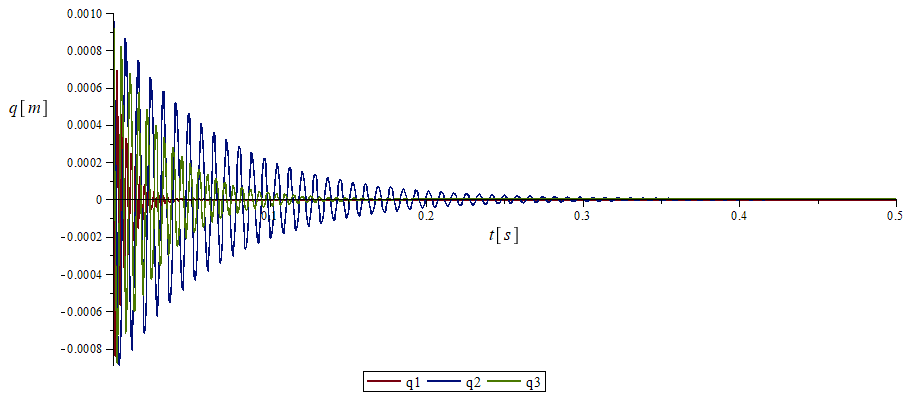
\includegraphics[width=\textwidth]{figs/q123_base_exemplo}
        \caption{Resultado MBS da base: translações q1, q2, q3}
        \label{fig::q123_base_exemplo}
    \end{subfigure}
    \quad %add desired spacing between images, e. g. ~, \quad, \qquad, \hfill
    % etc.
      %(or a blank line to force the subfigure onto a new line)
    \begin{subfigure}[b]{0.8\textwidth}
        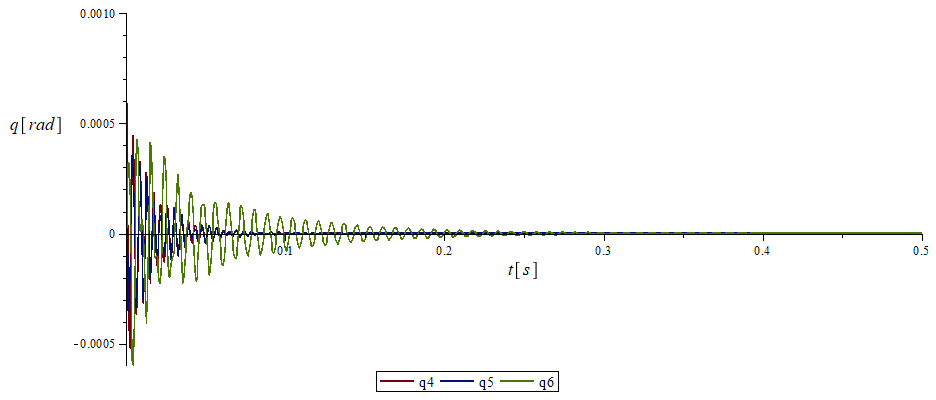
\includegraphics[width=\textwidth]{figs/q456_base_exemplo}
        \caption{Resultado MBS da base: rotações q4, q5, q6}
        \label{fig::q456_base_exemplo}
    \end{subfigure}
    \caption{Resultados dos primeiros 500~ms do deslocamento da base}
    \label{fig::res_qbase_exemplo}
\end{figure}

Note-se que, antes do tempo final da simulação, o sistema parece estar em
equilíbrio. O resultado de cada coordenada generalizada em $t=0,5~s$ é:
%
\begin{align*}
	q1(0,5) &= -0,20839\cdot 10^{-5}~m \\
	q2(0,5) &= 4,8952\cdot 10^{-8}~m \\
	q3(0,5) &= 8,4009 \cdot 10^{-12}~m \\
	q4(0,5) &= -1,6031\cdot 10^{-10}~rad \\
	q5(0,5)	&= -1,6260\cdot 10^{-11}~rad \\
	q6(0,5) &= 1,7857\cdot 10^{-8}~rad
\end{align*}
%
Verifica-se por este resultado que, no equilíbrio, os deslocamentos são
desprezíveis para o robô, tal que os valores máximos são da ordem de
$10^{-2}~mm$ em $q1$ e $10^{-11}~rad$ em $q5$.








% -.~.-.~.-.~.-.~.-.~.-.~.-.~.-.~.-.~.-.~.-.~.-
\section{Ensaio Experimental} \label{sec::experimento}

O amortecimento da estrutura que serve de base para o manipulador tem um papel
importante na dinâmica do sistema. Como foi demonstrado, o modelo MBS
acoplado robô-base requer como entrada os parâmetros de inércia, rigidez e amortecimento
da base. Os dados de inércia são facilmente obtidos pelo modelo CAD e a matriz
de inércia pela Análise por Elementos Finitos. Entretanto, estas
ferramentas não são capazes de fornecer informações sobre o amortecimento.
Modelar o amortecimento é um problema constante na engenharia de sistemas
mecânicos e continua um desafio.

O sistema robô-base não possui nenhum elemento com a finalidade específica de
controle ou absorção de vibrações. O que ocorre é o citado amortecimento
estrutural (seção~\ref{sec::amortecimento}), formado principalmente pelo
amortecimento do material \todo{Inlcuir referência no texto} e por atrito,
devido a folgas nos elementos de conexão, parafusos por exemplo.

Apesar de existir métodos para estimar o amortecimento material e de atrito
analiticamente, estes são adequados para estruturas muito simples e uniformes,
como vigas, placas ou corpos de prova. A estrutura que forma a base do robô é
relativamente muito complexa, possuindo diferentes materiais, conexões e formas,
o que torna impossível modelar analiticamente o amortecimento.

Logo, recorre-se ao método experimental para obter o amortecimento da base.
A vantagem é que por este método, obtém-se os parâmetros do comportamento total
da estrutura, não importando as infinitas interações internas dos materiais e de
atrito impossíveis de se medir ou quantificar individualmente.
Mais especificamente, o que importa é o comportamento do ponto de interação
robô-base.

Os parâmetros modais da base, associados aos  modos e frequências naturais de
vibração são obtidos por meio de um ensaio de vibrações.
A estrutura utilizada para o experimento é a denominada estrutura de testes,
Figura~\ref{fig::estrut_modelo_fisico}, sendo instrumentada com acelerômetros a
fim de se obter as acelerações associadas a cada um dos 6 graus de liberdade da
base, no ponto de interação com o robô. Um martelo instrumentado é utilizado
para excitar a base e obter as Funções de Resposta em Frequência (FRF's) de cada
grau de liberdade. Estes dados são utilizados para estimar os parâmetros modais:
modos de vibração, frequências naturais e amortecimentos.

Os resultados experimentais são então utilizados para calcular os parâmetros
$\alpha$ e $\beta$ da matriz de amortecimento proporcional.


\subsection{Bancada experimental e Instrumentação}

A base de testes é utilizada para os propósitos do ensaio e instrumentada com
acelerômetros. Deseja-se obter as acelerações de um ponto virtual, localizado no
centro da placa de fixação do robô. Este ponto representa a conexão teórica
entre a base e o manipulador, que restringe qualquer translação ou rotação
relativa entre eles.
Definindo-se um referencial fixo a este ponto, qualquer deslocamento e rotação
deste referencial transfere o mesmo movimento para o manipulador.

Levando isto em consideração, é preciso que as medidas coletadas do experimento
reflitam os deslocamentos deste ponto. Para isso, foram utilizados no total 7
acelerômetros uni-axiais, posicionados estrategicamente na placa de fixação do
robô. 

Os acelerômetros utilizados são modelo\ldots\todo{Incluir parágrafo descrição
dos acelerômetros}

A Figura~\ref{fig::acelerometos-base} apresenta a distribuição dos
acelerômetros na estrutura, onde são representados pelos pequenos cilindros
indicados, cuja direção de medição é a mesma do seu eixo, e o sentido positivo
sempre para fora da placa.

\begin{figure}[h]
	\centering 
 	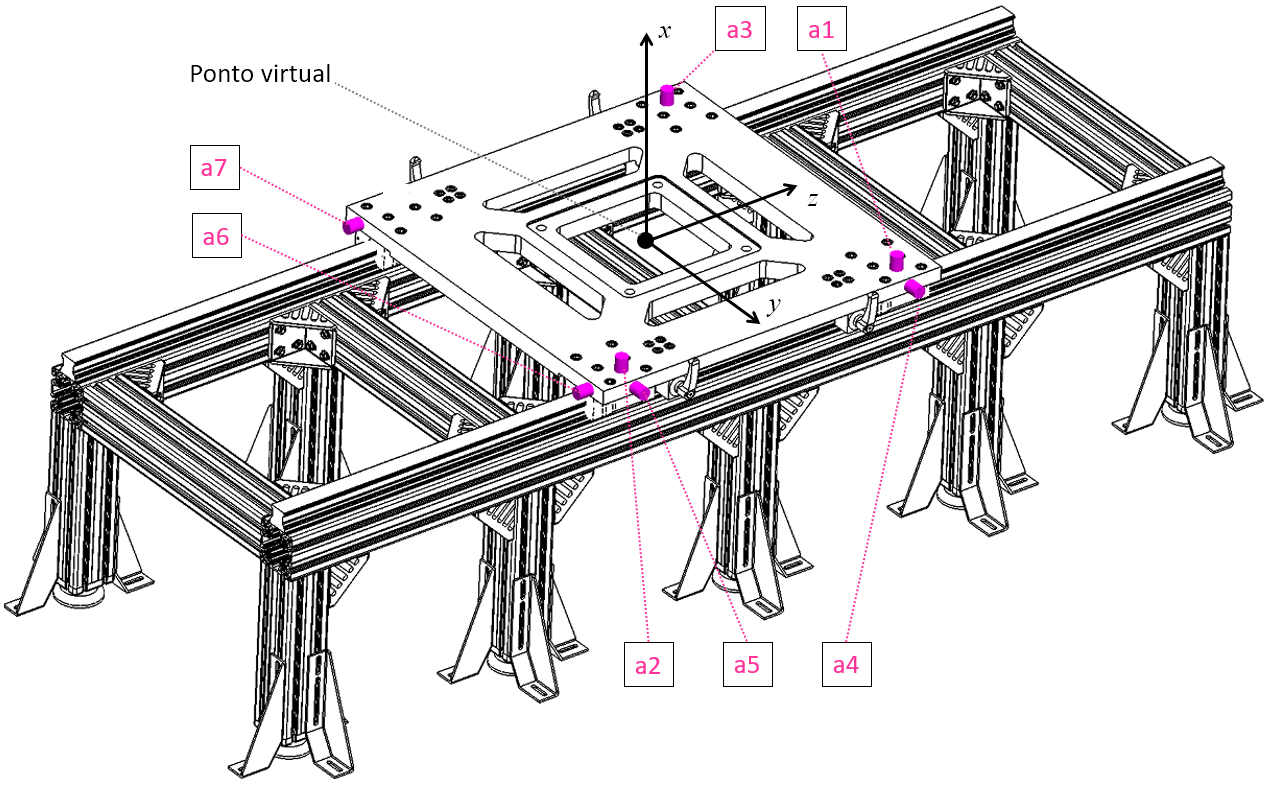
\includegraphics[width=0.95\textwidth]{figs/acelerometos-base}
 	\caption{Dsitribuição dos acelerômetros na base}
 	\label{fig::acelerometos-base}
\end{figure}

Assim como foi assumido no modelo para AEF da base, a placa de fixação do robô é
muito rígida em relação à estrutura de perfis de alumínio. Ou seja, as
deformações desta peça serão despezíveis e portanto a distância entre quaisquer
dois pontos sobre a placa permanecerá fixa no referencial local.
Isto permite a distribuição dos acelerômetros em qualquer ponto da placa
assumindo as acelerações são consideradas devido a movimento de corpo rígido e
não deformações elásticas da peça. 

Isto implica, que pode-se calcular a aceleração, em cada uma das 6 direções do
ponto virtual, a partir de relações aritméticas simples entre os sensores $a1$ a
$a7$. As acelerações lineares são indicadas pela variável $a$ e as
rotacionais por $\alpha$ seguidas de subíndice indicando sua orientação. Logo:
%
\begin{align}
	a_x &= \frac{a2+a3}{2} \\
	a_y &= \frac{a4+a5}{2} \\
	a_z &= - \frac{a6+a7}{2} \\
	\alpha_x &= \frac{a5-a4}{r1} \\
	\alpha_y &= \frac{a2-a1}{r1} \\
	\alpha_z &= \frac{a1-a3}{r2}
\end{align}
%
Onde $r1$ é a distância entre os acelerômetros $a1$ e $a2$, na direção $z$; e
$r2$ a distância entre os acelerômetros $a6$ e $a7$, direção $y$.

Note-se que é que as acelerações lineares são calculadas pela média entre dois
acelerômetros na mesma direção.
Já as acelerações angulares pela diferença entre os dois acelerômetros na mesma
direção, dividida pela distância, $r1$ ou $r2$ entre eles. Considere-se agora
que cada equação crie um sensor virtual, localizado no centro entre o par
calculado. Se a placa é rígida, pode-se considerar então que tais acelerações
são as mesmas correspondentes às do ponto central da placa. 

Tem-se portanto um vetor das acelerações generalizadas do referencial local da
placa, em que cada termo representa uma direção dos 6 gdl da base.
%
\begin{equation}
	\mathbf{a} = \left[ a_x, a_y, a_z, \alpha_x, \alpha_y, \alpha_z \right]
\end{equation}
%



Para aquisição dos dados experimentais são utilizadas duas placas NI-9234, da
fabricante National Instruments. Cada placa possui





\subsection{Aquisição dos dados experimentais}

\subsection{Tratamento dos dados}

\subsection{Cálculo dos parâmetros modais da estrutura}


% -.~.-.~.-.~.-.~.-.~.-.~.-.~.-.~.-.~.-.~.-.~.-
\section{Modelo acoplado robô e base} \label{sec::acoplado}

\subsection{Base rígida}

\subsection{Base flexível}


% -.~.-.~.-.~.-.~.-.~.-.~.-.~.-.~.-.~.-.~.-.~.-
\section{Estudos de casos para avaliação do método}\label{sec::casos}

\subsection{Trajetórias do efetuador}

\subsection{Base rígida}

\subsection{Base de testes}

\subsection{Base modular PRP}

\subsection{Base com pouca rigidez}
